\RequirePackage[l2tabu, orthodox]{nag}
%\documentclass[12pt]{article}
\documentclass[preprint,12pt,times]{elsarticle}

\biboptions{sort&compress,comma,square}

% \usepackage{url}

% \usepackage[linesnumbered,lined,commentsnumbered,ruled]{algorithm2e}
%\usepackage{amssymb}
\usepackage{amsmath}
%\usepackage{amsfonts}
\usepackage{bm}
%\usepackage{bbm}
%\usepackage{caption}
\usepackage{xcolor}
%\usepackage{geometry}
%\usepackage{graphicx}
%\usepackage[colorlinks,linkcolor=blue,citecolor=blue,urlcolor=blue]{hyperref}
\usepackage{listings}
\lstset{ %
   backgroundcolor=\color{white},   % choose the background color; you must add \usepackage{color} or \usepackage{xcolor}
   basicstyle=\small,        % the size of the fonts that are used for the code
   breakatwhitespace=false,         % sets if automatic breaks should only happen at whitespace
   breaklines=false,                 % sets automatic line breaking
   captionpos=b,                    % sets the caption-position to bottom
   %commentstyle=\color{mygreen},    % comment style
   deletekeywords={...},            % if you want to delete keywords from the given language
   escapeinside={\%*}{*)},          % if you want to add LaTeX within your code
   extendedchars=false,              % lets you use non-ASCII characters; for 8-bits encodings only, does not work with UTF-8
   frame=single,	                   % adds a frame around the code
   keepspaces=true,                 % keeps spaces in text, useful for keeping indentation of code (possibly needs columns=flexible)
   keywordstyle=\color{blue},       % keyword style
   language=C++,                 % the language of the code
   otherkeywords={*,...},           % if you want to add more keywords to the set
   numbers=left,                    % where to put the line-numbers; possible values are (none, left, right)
   numbersep=5pt,                   % how far the line-numbers are from the code
   numberstyle=\tiny\color{gray}, % the style that is used for the line-numbers
   rulecolor=\color{black},         % if not set, the frame-color may be changed on line-breaks within not-black text (e.g. comments (green here))
   showspaces=false,                % show spaces everywhere adding particular underscores; it overrides 'showstringspaces'
   showstringspaces=false,          % underline spaces within strings only
   showtabs=false,                  % show tabs within strings adding particular underscores
   stepnumber=2,                    % the step between two line-numbers. If it's 1, each line will be numbered
%   stringstyle=\color{mymauve},     % string literal style
   tabsize=2,	                   % sets default tabsize to 2 spaces
   title=\lstname                   % show the filename of files included with \lstinputlisting; also try caption instead of title
}
%\usepackage{layouts}
%\usepackage{mathrsfs}
%\usepackage{pgfkeys,pgfmath,pgfcore}
%\usepackage{srcltx}
%\usepackage[labelformat=simple]{subcaption}
%\usepackage{xspace}
\usepackage[linesnumbered,lined,commentsnumbered,ruled]{algorithm2e}

\usepackage[format=plain,indention=.5cm]{caption}
\usepackage[labelformat=simple]{subcaption}
\renewcommand\thesubfigure{(\alph{subfigure})}

%\renewcommand{\thetable}{\arabic{table}}
%\captionsetup[table]{labelformat=simple, labelsep=colon}

%\pgfkeys{/pgf/number format/.cd,1000 sep={}}

%% see http://tex.stackexchange.com/questions/2441/how-to-add-a-forced-line-break-inside-a-table-cell
%\newcommand{\specialcell}[2][c]{%
%  \begin{tabular}[#1]{@{}c@{}}#2\end{tabular}}

% put your own definitions here:
% \renewcommand\thesubfigure{(\alph{subfigure})}
\def\gz  #1{           \mbox{$\boldsymbol{#1}$}}
% \DeclareMathAlphabet{\bsf}{OT1}{cmss}{bx}{n}
% \def\msf  #1{           \mbox{\!\!      $\sf #1$}}
\def\Grad #1 {{\rm Grad} #1}
\def\grad #1 {{\rm grad} #1}
\def\Div {\mbox{Div\,}}
\def\div {\mbox{div\,}}
\def\d {\,\mbox{d}}
\def\D {\,\mbox{D}}
% \newcommand{\norm}[1]{\left\lvert #1 \right\rvert}
%\newcommand\normDouble[1]{\left\lVert#1\right\rVert}
%\newcommand{\normXY}[1]{\lvert #1 \rvert_{2d}}
%\newcommand{\dbracket}[1]{\left[\!\!\left[ #1 \right]\!\!\right]}

\def\mcl  #1{               {\cal #1}}
%\def\bcl  #1{\mbox{\boldmath$\cal #1$}}

%\DeclareMathOperator{\det}{det}
\DeclareMathOperator{\trace}{tr}
\newcommand{\diff}{\mathop{}\!\mathrm{d}}


\begin{document}

\begin{frontmatter}
  \title{
  A matrix-free approach for finite-strain hyperelastic problems using geometric multigrid
  }

  \author[a]{Denis Davydov\corref{cor}}
  \ead{denis.davydov@fau.de}

  \author[a]{Jean-Paul Pelteret}
  \ead{jean-paul.pelteret@fau.de}

  \author[b]{Daniel Arndt}
  \ead{daniel.arndt@iwr.uni-heidelberg.de}

  \author[a]{Paul Steinmann}
  \ead{paul.steinmann@fau.de}

  \cortext[cor]{Corresponding author.}

  \address[a]{Chair of Applied Mechanics,
  Friedrich-Alexander-Universit\"{a}t Erlangen-N\"{u}rnberg,
  Egerlandstr.\ 5, 91058 Erlangen, Germany}

  \address[b]{Interdisciplinary Center for Scientific Computing (IWR),
      Heidelberg University,
      Im Neuenheimer Feld 205,
      69120 Heidelberg,
      Germany}


  \begin{abstract}
    The performance of finite element solvers on modern computer architectures is typically memory bound.
    The main cause for this is that loading matrix elements is significantly slower than performing the arithmetic operations when solving the problem.
    In order to improve the performance of the iterative solver, so-called matrix-free methods are
    widely adopted in fluid mechanics community, where the matrix vector products are formed on-the-fly.

    In this work, we advance the application of matrix-free approaches to problems in solid mechanics.
    We propose and numerically investigate different implementations of the finite-strain hyper-elastic tangent operator.
    In order to improve the convergence of iterative solvers, we also propose a way to construct level tangent operators
    and employ them to define a geometric multigrid preconditioner.
    Our implementation employs MPI and Intel Threading Building Blocks parallelization and SIMD vectorization.
    The performance of the matrix-free operator and the geometric multigrid preconditioner is compared to the matrix-based implementation with an algebraic multigrid preconditioner for a representative numerical example of heterogeneous hyper-elastic material in two and three dimensions.
  \end{abstract}


  \begin{keyword}
      adaptive finite element method \sep
      geometric multigrid \sep
      finite-strain \sep
      matrix-free \sep
      hyperelasticity
  \end{keyword}

  \end{frontmatter}

\section{Introduction}

The performance of finite element (FEM) solvers on modern computer architectures is typically memory bound.
The main cause for this is that loading matrix elements is significantly slower than performing the arithmetic operations when solving the problem.
In order to improve the performance of the iterative solver, so-called matrix-free methods are
widely adopted in fluid mechanics community, where the matrix vector products are formed on-the-fly \cite{kronbichler12,May2015, Krank2017, Brown2010, Gmeiner2016}. Such methods can also be efficiently implemented on GPUs \cite{Abdelfattah2016}.

To the best of our knowledge, the matrix-free methods are not yet widely adopted within the solid mechanics community.
We are only aware of a single paper in preparation that deals with small strain linear elasticity \cite{Clevenger2018} and a master thesis of a student of two of the authors \cite{Mentler2017}.
A possible reason is that tangent operators (coming from linearization of the nonlinear balance equations) are
more elaborate as compared to the fluid mechanics and it is not obvious whether the matrix-free methods can be advantageous in this case. Another reason could be the smoothness of the underlying solution. FEM with linear or quadratic elements (to avoid locking) are often adopted in solid mechanics community. However we note that large scale computations with $10^{12}$ unknowns even with linear FEM inevitably require matrix-free approach as there is simply not enough memory to store the sparse tangent matrix \cite{Gmeiner2016}. Therefore we believe that for large scale computations in solid mechanics it is crucial to adopt matrix-free approaches and develop efficient multigrid solvers.

In this work, we advance the application of matrix-free approaches to problems in solid mechanics.
We propose and numerically investigate different implementations of the finite-strain hyper-elastic tangent operator.
In order to improve the convergence of iterative solvers, we also propose a way to construct level tangent operators
and employ them to define a geometric multigrid preconditioner.
Our implementation employs MPI and Intel Threading Building Blocks parallelization and SIMD vectorization.

The paper is organized as follows. In Section \ref{sec:theory} we briefly introduce partial differential equations of finite-strain solid mechanics. Sections \ref{sec:fe} and \ref{sec:mf} cover the finite element discretization and the proposed matrix-free operator evaluation approaches. In Section \ref{sec:gmg} we propose a geometric multigrid preconditioner suitable for finite-strain linear elasticity. The performance of the matrix-free operator and the geometric multigrid preconditioner is compared to the matrix-based implementation with an algebraic multigrid preconditioner for a representative numerical example of heterogeneous hyper-elastic material in two and three dimensions in Section \ref{sec:example}. Summary is presented in Section \ref{sec:summary}.

\section{Theoretical background}
\label{sec:theory}

In this section we briefly summarize balance equations of fine-strain hyperelastic continuum.

{\color{red}
TODO: JP please adjust this part to your liking
}

Deformation of the body $\mcl B$ from the reference configuration $\mcl B_0$ to the current configuration $\mcl B_t$
is defined via the mapping $\gz x = \gz \varphi (\gz X,t)$.
The displacement field reads $\gz u = \gz x - \gz X$.
%
Linear deformation map is assumed
$\d \gz x = \gz F \cdot \d \gz X$,
where $\gz F := \Grad \, \gz \varphi \equiv \gz I + \Grad \, \gz u$ is the deformation gradient.
For conservative systems without the volumetric load the total potential energy functional $\mcl E$ is introduced as
\begin{align}
\mcl E =
\int_{\mcl B_0} \mcl \psi(\gz F; \gz X) \d V \,
- \int_{\partial \mcl B_0^N} \gz T \cdot \gz u \d S \, ,
\end{align}
where $\gz T$ is the prescribed loading at the Neumann part of the boundary $\partial \mcl B_0^N$ in reference configuration, $\mcl \psi$ denotes the strain-energy per unit reference volume and $\gz u$ should satisfy the prescribed Dirichlet boundary conditions $\gz u = \gz u^D$ on $\partial \mcl B_0^D := \partial \mcl B_0 \setminus \partial \mcl B_0^N \neq \emptyset $.

The principal of stationary potential energy requires that at the equilibriums the directional derivative with respect to the displacement $\gz u$
\begin{align}
\delta \mcl E =
\frac{\d}{\d \epsilon} \mcl E (\gz u + \epsilon \delta \gz u) \Bigr\rvert_{\epsilon=0}  = 0 \, .
\label{eq:stationary}
\end{align}
vanishes for all directions $\delta \gz u$ which satisfy homogeneous Dirichlet boundary conditions.
%
This leads to the following non-linear equation
\begin{align}
F(\gz u, \delta \gz u) =
\int_{\mcl B_0} \gz P : \Grad \, \delta \gz u \d V \,
-
\int_{\partial \mcl B_0^N} \gz T \cdot \delta \gz u \d S
= 0 \, ,
\end{align}
where $\gz P := \partial \mcl \psi / \partial \gz F$ is the Piola stress.


\subsection{Linearization}

{\color{red}TODO: linearize and show how tangent look like.
Also show what it boils down in the case of small strain.
}

\subsection{Constitutive modelling}

Neo-Hookean model
\begin{gather}
\psi \left( \mathbf{C} \right)
  = \frac{\mu}{2} \left[ \trace{\mathbf{C}} - \trace{\mathbf{I}} - 2 \ln\left( J \right) \right]
  + \lambda \ln^{2}\left( J \right)
\end{gather}
where $\mu$ and $\lambda$ respectively denote the shear modulus and Lam\'{e} parameter,
and the volumetric Jacobian $J = \det\left(\mathbf{F}\right) = \sqrt{\det\left(\mathbf{C}\right)}$.
\begin{gather}
\frac{d \psi \left( \mathbf{C} \right)}{d \mathbf{C}}
  = \frac{\mu}{2} \mathbf{I} - \frac{1}{2} \left[ \mu - 2\lambda\ln\left( J \right) \right] \mathbf{C}^{-1}
\end{gather}
\begin{gather}
\frac{d^{2} \psi \left( \mathbf{C} \right)}{d \mathbf{C} \otimes d \mathbf{C}}
  = \frac{1}{2}\left[ \mu - 2\lambda\ln\left( J \right) \right] \left[ - \frac{d \mathbf{C}^{-1}}{d \mathbf{C}} \right]
  + \frac{\lambda}{2} \mathbf{C}^{-1} \otimes \mathbf{C}^{-1}
\end{gather}

Denoting $\chi\left( \bullet \right)$ as the Piola transformation, which implies
\begin{gather}
\chi\left( \mathbf{A} \right)_{ij}
  = F_{iA} A_{AB} F_{jB} \\
\chi\left( \boldsymbol{\mathcal{A}} \right)_{ijkl}
  = F_{iA} F_{jB} \mathcal{A}_{ABCD} F_{kC} F_{lD}
\end{gather}
for rank-2 and rank-4 tensors $\mathbf{A}$ and $\boldsymbol{\mathcal{A}}$, then the Kirchhoff stress and its associated material tangent are
\begin{gather}
\boldsymbol{\tau}
  \equiv J \boldsymbol{\sigma}
  = \chi\left( 2 \frac{d \psi \left( \mathbf{C} \right)}{d \mathbf{C}} \right)
  = \mu \mathbf{b} - \left[ \mu - 2\lambda\ln\left( J \right) \right] \mathbf{I}
\end{gather}
and
\begin{gather}
J \boldsymbol{\mathcal{C}}
  = \chi\left( 4 \frac{d^{2} \psi \left( \mathbf{C} \right)}{d \mathbf{C} \otimes d \mathbf{C}} \right)
  = 2 \left[ \mu - 2\lambda\ln\left( J \right) \right] \boldsymbol{\mathcal{S}}
  + 2 \lambda \mathbf{I} \otimes \mathbf{I}
\end{gather}
where $\boldsymbol{\mathcal{S}}$ is the fourth-order symmetric identity tensor.
The action that $J \boldsymbol{\mathcal{C}}$ performs when contracted with an arbitrary rank-2 symmetric tensor is therefore
\begin{gather}
J \boldsymbol{\mathcal{C}} : \left( \bullet \right)
  = 2 \left[ \mu - 2\lambda\ln\left( J \right) \right] \left( \bullet \right)
  + 2 \lambda \trace\left( \bullet \right) \mathbf{I}
\end{gather}

\section{Finite Element discretization}
\label{sec:fe}

We now introduce a FE triangulation $\mathcal{T}^h$ of $\mcl B_0$ and
the associated FE space of continuous piecewise elements of a fixed polynomial degree. % : $V^h \subset H^1 (\mcl B_0)$.
The deformation map are given in a
a vector space spanned by standard vector--valued FE basis functions $\gz N^i(\gz x)$ (e.g. polynomials with local support):
\begin{alignat}{2}
       \gz \varphi^h &=:  \sum_{i \in \mcl I_\varphi}       \varphi_i \gz N^i_\varphi (\gz X) \quad \quad \quad
\delta \gz \varphi^h &&=: \sum_{i \in \mcl I_\varphi} \delta \varphi_i \gz N^i_\varphi (\gz X) \,,
\end{alignat}
where superscript $h$ denotes that this representation is related to the FE mesh with size function $h(\gz X)$ and $\mcl I_\varphi$ is the sets of unknown degrees of freedom (DoF).
For the sake of this study $\gz N^i_\varphi (\gz X)$ are such that only one component of the vector-valued shape function is non-zero for each $i$.

\section{Matrix-free operator evaluation}
\label{sec:mf}
Classically the approach for finding a discrete solution to a linearized partial differential equation can be described as follows:
First, ansatz spaces and a suitable bilinear form is defined. Then, a matrix and force vector corresponding to the discretization are assembled.
Finally, a direct or iterative solver is used to solve the linear system for the discretized solution.
On modern computer architectures however, it turns out that loading data is significantly slower than performing the arithmetic operations when solving.
For this reason, recent implementations often focus on so-called matrix-free approaches. The idea is to perform the operations in the solver on-the-fly
rather than loading matrix elements from memory.
For iterative solvers, this is possible since it is sufficient to compute matrix vector products. More precisely, the linear system corresponding to a bilinear form
$a\colon V_h\times V_h\to\mathbb{R}$ and right-hand side $f\colon V_h\to\mathbb{R}$ defined with respect to the ansatz space $V_h$ can be represented by
\begin{align*}
 &&a(v,u) &= f(v) && \forall v\in V_h\\
 \Longleftrightarrow &&a(\varphi_i, u) &= f(\varphi_i) && \forall \varphi_i \\
 \Longleftrightarrow &&\sum_j a(\varphi_i,\varphi_j) u_j &= f(\varphi_i) && \forall \varphi_i \\
 \Longleftrightarrow &&A x &= b
\end{align*}
where $A_{i,j}=a(\varphi_i, \varphi_j)$ and $b_i= f(\varphi_i)$.
Thus, the matrix-vector product $Ax$ can be expressed by
\begin{align*}
 (Ax)_i &= \sum_j a(\varphi_i,\varphi_j) x_j \\
        &= \sum_K\sum_q \sum_j \tilde{a}_K(\varphi_i,\varphi_j)(x_q) x_j w_q
\end{align*}
where in the last step $\tilde{a}_K(\varphi_i,\varphi_j)$ is a representation for the evaluation of the bilinear in one quadrature point and a quadrature rule is used.
For the sake of demonstration, let us assume $A$ represents a mass matrix. In this case, it holds
\begin{align*}
 \tilde{a}_K(\varphi_i,\varphi_j)(x_q) = \varphi_i(x_q)\varphi_j(x_q).
\end{align*}
Further assuming that the number of the one-dimensional quadrature points $n$ matches the degree of the ansatz space plus one, the evaluation of all the shape functions ($n^d$)
in all quadrature points ($n^d$) has complexity $\mathcal{O}(n^{2d})$ in case we consider a problem in $d$ space dimensions. For the total matrix-vector product we get $\mathcal{O}(2n^{2d})$
and this is the same as for a regular matrix-vector where the entries are already precomputed. Assuming tensor product ansatz spaces and a tensor product quadrature rule, we can actually do better
than that. Indeed, the evaluation of all the shape functions in all the ansatz points can be rewritten as
\begin{lstlisting}
template<int k, int q>
void evaluate_dof_vector_in_all_quadrature_points
  (const double u[k][k][k],
   const double phi[k][q],
   double return_value[q][q][q])
{
  double tmp1[k][k][q] {};
  for (int i1=0; i1<k; ++i1)
    for (int i2=0; i2<k; ++i2)
      for (int q3=0; q3<q; ++q3)
        for (int i3=0; i3<k; ++i3)
          tmp1[i1][i2][q3] += u[i1][i2][i3]*phi[i3][q3];

  double temp2[k][q][q] {};
  for (int i1=0; i1<k; ++i1)
    for (int q3=0; q3<q; ++q3)
      for (int q2=0; q2<q; ++q2)
        for (int i2=0; i2<k; ++i2)
          tmp2[i1][q2][q3] += tmp1[i1][i2][q3]*phi[i2][q2];

  for (int q2=0; q2<q; ++q2)
    for (int q3=0; q3<q; ++q3)
      for (int q1=0; q1<q; ++q1)
        for (int i1=0; i1<k; ++i1)
  return_value[q1][q2][q3] += tmp2[i1][q2][q3]*phi[i1][q1];
}
\end{lstlisting}
in three space dimensions. In general, this reordering reduces the arithmetic complexity to $\mathcal{O}(dn^{d+1})$ and is called sum factorization.
Hence, we can expect that such a matrix-free approach is faster than a regular matrix-base especially for 3D and high polynomial degree.
More information on techniques to increase the computational density can be found in \cite{kronbichler12,vos10}.
We briefly note that the SIMD vectorization is applied at the element level, that is the operator is applied simultaneously on several several elements (called ``block'') whereas the shared memory parallelization using Intel Threading Building Blocks is adopted at the element blocks.

Given that the matrix-free operators are applied on-the-fly, it's crucial to find a good balance between pre-calculation of certain values (caching) and performance of the algorithm.
Below we propose three algorithms to implement tangent operator of finite-strain linear elasticity using matrix-free approach, that employ different caching strategies.
%
In order to obtain gradients with respect to the deformed configuration we adopted \textit{MappingQEulerian} class from \texttt{deal.II} library.
In addition to the standard mapping from the reference (unit / isoparametric) element to the element in real space, this class adds mapping to the deformed configuration given a displacement field.
%
Due to the specifics of matrix-free operator evaluation implemented in \texttt{deal.II}, when performing contraction with gradient of shape functions in current (deformed) configuration, the integration is also done over the deformed configuration. Therefore in order to arrive at the integral in undeformed configuration, additionally we have to divide by Jacobian $J$ of the mapping at a given quadrature point.

\begin{algorithm}[!ht]
  \SetKwInOut{Input}{Given}
  \SetKwInOut{Output}{Return}
  \Input{RHS FE vector $\gz x$, current FE solution $\gz u$,
  cacheed $c_1 := \mu - 2 \lambda \log(J)$ for each cell and quadrature point}
  \Output{action of the FE tangent on $\gz x$}
  \ForEach{ element $K \in \Omega^h$ }{
        \ForEach{quadrature point $q$ on $K$}{
          evaluate $\gz \nabla_X \gz u^h$ \tcp*{2nd order}
          evaluate $\gz F = \gz I + \gz \nabla_X \gz u^h$ \tcp*{2nd order}
          evaluate $J = \rm{det}(\gz F)$ \tcp*{scalar}
          evaluate $\gz b = \gz F \cdot \gz F^T$ \tcp*{2nd order symmetric}
          evaluate $\gz g := \gz \nabla \gz x$ \tcp*{2nd order}
          evaluate $\gz \tau = \mu \gz b - c_1 \gz I$ \tcp*{2nd order symmetric}
          evaluate $\boldsymbol{\mathcal{G}} \gz g = \gz g \cdot \gz \tau/J$ \tcp*{2nd order}
          ``submit'' contraction $\gz \nabla \gz N_i : \boldsymbol{\mathcal{G}} \gz g$\;
          evaluate $\gz g_s := \gz \nabla_{sym} \gz x$ \tcp*{2nd order symmetric}
          evaluate $\boldsymbol{\mathcal{C}}\gz g_s = \left[2 c_1 \gz g_s + 2 \lambda\, \rm{tr}( \gz g_s) \gz I \right]/J$ \tcp*{2nd order symmetric}
          ``submit'' contraction $\gz \nabla_{sym} \gz N_i : \boldsymbol{\mathcal{C}}\gz g_s$ \;
        }
  }
  \caption{Matrix-free tangent cell operator: scalar cache}
  \label{alg:mf_scalar}
\end{algorithm}

Algorithm \ref{alg:mf_scalar} caches a single scalar which involves logarithm of Jacobian -- a computationally demanding operation compared to addition and multiplications. As evident from Section \ref{sec:theory}, in order to apply the operator we need to re-evaluate Kirchhoff stress at each quadrature point. This in turn requires evaluation of deformation gradient $\gz F$ and therefore gradients with respect to the undeformed configuration.

\begin{algorithm}[!ht]
  \SetKwInOut{Input}{Given}
  \SetKwInOut{Output}{Return}
  \Input{RHS FE vector $\gz x$,
  cached
  $c_1 := 2\left[\mu - 2 \lambda \log(J)\right]/J$,
  $c_2 := 2\lambda/J$ and $\gz \tau/J$ for each cell and quadrature point}
  \Output{action of the FE tangent on $\gz x$}
  \ForEach{ element $K \in \Omega^h$ }{
        \ForEach{quadrature point $q$ on $K$}{
          evaluate $\gz g := \gz \nabla \gz x$ \tcp*{2nd order}
          evaluate $\boldsymbol{\mathcal{G}}\gz g = \gz g \cdot \left[\gz \tau/J \right]$ \tcp*{2nd order}
          ``submit'' contraction $\gz \nabla \gz N_i : \boldsymbol{\mathcal{G}} \gz g$ \;
          evaluate $\gz g_s := \gz \nabla_{sym} \gz x$ \tcp*{2nd order symmetric}
          evaluate $\boldsymbol{\mathcal{C}} \gz g_s = c_1 \gz g_s + c_2 \, \rm{tr}(\gz g_s) \gz I$ \tcp*{2nd order symmetric}
          ``submit'' contraction $\gz \nabla_{sym} \gz N_i : \boldsymbol{\mathcal{C}} \gz g_s $ \;
        }
  }
  \caption{Matrix-free tangent cell operator, variant 1: cache second order Kirchhoff stress $\gz \tau$ and thereby avoid the need to evaluate refential quantities like $\gz F$ at runtime.}
  \label{alg:mf_tensor2}
\end{algorithm}

In order to avoid re-calculation of the Kirchhoff stress, Algorithm \ref{alg:mf_tensor2} caches its value for each element and quadrature point. This also avoid the need to evaluate gradients of displacement field with respect to the undeformed configuration. This algorithm utilize the chosen constitutive relationship and therefore the action of the material fourth order tangent $\boldsymbol{\mathcal{C}}$ on the second order symmetric tensor $\gz g_s$ can be evaluated by taking a linear combination this tensor and its trace times identity tensor. To that end we also cache two scalars that depend on the Jacobian $J$.

\begin{algorithm}[!ht]
  \SetKwInOut{Input}{Given}
  \SetKwInOut{Output}{Return}
  \Input{RHS FE vector $\gz x$,
  cached $\gz \tau/J$ and $\boldsymbol{\mathcal{C}}$ for each cell and quadrature point}
  \Output{action of the FE tangent on $\gz x$}
  \ForEach{ element $K \in \Omega^h$ }{
        \ForEach{quadrature point $q$ on $K$}{
          evaluate $\gz g := \gz \nabla \gz x$ \tcp*{2nd order}
          evaluate $\boldsymbol{\mathcal{G}} \gz g = \gz g \cdot \left[\gz \tau/J\right]$ \tcp*{2nd order}
          ``submit'' contraction $\gz \nabla \gz N_i : \boldsymbol{\mathcal{G}} \gz g$\;
          evaluate $\gz g_s := \gz \nabla_{sym} \gz x$ \tcp*{2nd order symmetric}
          evaluate $\boldsymbol{\mathcal{C}}\gz g_s = \boldsymbol{\mathcal{C}}\gz : \gz g_s$ \tcp*{2nd order symmetric}
          ``submit'' contraction $\gz \nabla_{sym} \gz N_i : \boldsymbol{\mathcal{C}}\gz g_s$ \;
        }
  }
  \caption{Matrix-free tangent cell operator: cache fourth order material tangent $\boldsymbol{\mathcal{C}}$ and Kirchhoff stress $\gz \tau$.}
  \label{alg:mf_tensor4}
\end{algorithm}

Finally Algorithm \ref{alg:mf_tensor4} represents the most general algorithm which does not assume specific constitutive relationship.
Clearly in this case we have to cache the fourth order symmetric tensor $\boldsymbol{\mathcal{C}}$ for each element and quadrature point and perform the double contraction with the second-order symmetric tensor on-the-fly.

\section{Geometric multigrid preconditioning}
\label{sec:gmg}

Efficient and scalable matrix-vector products is not enough to obtain a method with linear scaling with respect to the number of unknown DoFs $N$.
Efficiency of standard iterative solvers deteriorate for large systems of linear equations.
It has been widely accepted that the geometric multigrid (GMG) preconditioners \cite{Bramble1990, Briggs2000, Janssen2011,May2015} can greatly improve the performance of iterative solvers by smoothing the defect on a hierarchy of levels.
As a result the number of iterations for convergence becomes independent of the number of mesh refinements and thus leads to the $\mathcal O (N)$ solution method. For further information about geometric multigrid methods we refer the reader to \cite{Briggs2000,Hackbusch1985,Wesseling1992}.

For this work we adopt the matrix-free level operators within the GMG and Chebyshev pre- and post-smoothing on each level. Given a generally heterogeneous non-linear material, definition of transfer operations (restriction and prolongation) and level operators is not trivial. One approach is to start from an arbitrary heterogeneous material at the fine scale and employ homogenization theory \cite{Suquet1985, Hill1972,Hashin1983,Castaneda1997} to design specific transfer operators \cite{Miehe2007}\footnote{
  We note that this approach is limited to the case where for each quadrature point within an element the fourth order tangent operator is the same.
}.
In this approach the fine-scale displacement is decomposed into long-wave and short-wave contributions by additive split, where the former is associated to the homogeneous response of a patch of elements and the latter represents fluctuations due to the heterogeneous structure of the patch. In the case of a homogeneous patch, the transfer operators reduce to the standard geometric transfer. Based on this observation we adopt the following approach. It is assumed that the mesh at the coarsest level can accurately describe the heterogeneous fine-strain elastic material. In this case the restriction and prolongation operations for patches of elements are always performed for the same material and thus admits usage of standard geometric transfer operators. We define the level operators as follows. Recall that the fine scale tangent is obtain by linearization around the current displacement field $\gz u^h$. We then restrict this displacement field to multigrid levels $\{l\}$ and evaluate tangent operators using the matrix-free algorithms from Section \ref{sec:mf}. Essentially level operators correspond to the linearization around smoothed representation of displacement field.
Note that by doing so the operator (tangent) $K^{l+1}$ on level $l+1$ is not directly related to the operator (tangent) $K^{l}$ on level $l$ via $K^{l+1}=I^{l+1}_{l}  K^l I^l_{l+1}$, where $I^l_{l+1}$ and $I^{l+1}_l$ are prolongation (coarse-to-fine) and restriction (fine-to-coarse) operators, respectively.
Finally, at the coarsest level we adopt CG solver which shall reduce residual by three orders of magnitude within at most hundred of steps.
The classical multigrid V-cycle approach with two pre- and post-smoothing is adopted. For other approaches that combine homogenization and multigrid methods for small strain elastic materials, see \cite{Bayreuther2003,Fish1995}.

\section{Numerical examples}
\label{sec:example}

In this section we apply the proposed matrix-free operator algorithms for finite-strain hyper-elastic material as well as the geometric multigrid preconditioner to a benchmark problem from \cite{Miehe2007}. Coarse mesh for 2D and 3D problems is depicted in Figure \ref{fig:miehe}. The 2D material consists of a matrix (depicted in blue), a hole and two spherical inclusions (depicted in red). The size of the square domain is $10^{-3} \rm{mm}$.
The matrix material is taken to have Poisson's ratio of $0.3$ and shear modulus $\mu=0.4225 \times 10^6\, \rm{N/mm^2}$. The inclusion is take to be $100$ times harder.
The 3D material is obtained by extrusion in the third direction.
Note that a relatively coarse mesh is adopted at the coarsest multigrid level, however the geometry of inclusions is captured accurately by employing manifold description of the boundaries and interfaces.
Both domains are fixed at the bottom surface and the distributed load is applied at the top in $(1,0)$ and $(1,1,0)$ direction for 2D and 3D problems, respectively.
The load of $0.5\,\rm{N}$ is applied in 5 steps. The displacement tolerance for Newton update is taken to be $10^{-5}$ whereas the relative and absolute tolerances for forces $10^{-8}$. The relative convergence criteria for linear solver is $10^{-6}$.
%
Figure \ref{fig:miehe_gmg} illustrates the multigrid mesh for the 2D problem after two global refinements.
%
The benchmark calculations are performed for 2D and 3D problems with various combination of polynomial degrees and number of global refinements, see Tables \ref{tab:input_parameters_2d} and \ref{tab:input_parameters_3d}.
%
We are interested in the following metrics:
(i) walltime per DoF of matrix-vector multiplication;
(ii) memory requirement per DoF;
(iii) average number of CG iterations throughout the whole run (i.e. each Newton-Raphson iteration and each loading step);
(iv) walltime per DoF of CG solver;
%
The results of the matrix-free approach with geometric-multigrid preconditioner are compared to the matrix-based approach with algebraic multigrid (AMG) preconditioner using Trilinos \cite{Heroux2005} library.
The aggregation threshold for AMG is taken as $10^{-4}$.
Computations are done on a single node of two clusters.
A node on ``Emmy'' cluster has two Xeon 2660v2 ``Ivy Bridge'' chips (10 cores per chip + SMT) running at 2.2 GHz with 25 MB Shared Cache per chip and 64 GB of RAM. Intel compilers version 18.03 with flags ``-O3 -march=native'' and Intel MPI version 18.03 are used.
The ``IWR'' results were obtained ona single machine with eight Xeon E7-8870 ``Sandy Bridge'' chips (10 cores per chip  + SMT) running at 2.4 GHz with 30 MB Shared Cache per chip. For the simulation, GNU 8.1.0 with flags ``-O3 -march=native'' and OpenMPI 3.0.0 were used.

Figures \ref{fig:benchmark_miehe_Emmy} and \ref{fig:benchmark_miehe_IWR} show the results of the benchmarks as performed on the two clusters.
As expected the matrix-vector multiplication becomes very expensive for higher order discretization for matrix-based approaches.
The matrix-free implementation is faster than the matrix-based counterpart already for cubic Lagrangian basis in 2D and quadratic in 3D.
Figures \ref{fig:benchmark_miehe_Emmy_vmult2}, \ref{fig:benchmark_miehe_Emmy_vmult3}, \ref{fig:benchmark_miehe_IWR_vmult2} and \ref{fig:benchmark_miehe_IWR_vmult3} clearly shows the influence of different caching strategies.
Two conclusions can be drawn: scalar caching implementation is the most time consuming at each step we additionally evaluate the gradient of displacement field in reference configuration, required to evaluate the Kirchhoff stress $\gz \tau$. On another hand there is little difference between the approach where the fourth order material tangent tensor is cached (``tensor4'') and the one where we only cache the second order Kirchhoff tensor and use the chosen hyper-elastic constitutive equation to efficiently implement the action of the material tangent on the second order symmetric tensor.
This indicates that the time savings we get from the latter approach are insignificant within the complete matrix-free operator implementation.
Consequently we can apply matrix-free approach to any fine-strain material model by caching the fourth order material tangent in addition to the Kirchhoff stress and expect this to be faster than the matrix-based implementation.

As outlined in the introduction, it is not only the performance of the matrix-free vector multiplication, but also the memory requirement to store a sparse matrix which is the driving force behind the matrix-free methods.
Figures \ref{fig:benchmark_miehe_Emmy_memory2}, \ref{fig:benchmark_miehe_Emmy_memory3}, \ref{fig:benchmark_miehe_IWR_memory2} and \ref{fig:benchmark_miehe_IWR_memory3} show that even with caching of one fourth order symmetric tensor and one second order tensor at each quadrature point, the matrix-free approach takes much less memory than its matrix-based counterpart.

Next we evaluate the performance of the proposed geometric multigrid preconditioner. First we consider the number of CG iterations.
Figures \ref{fig:benchmark_miehe_Emmy_cg2}, \ref{fig:benchmark_miehe_Emmy_cg3}, \ref{fig:benchmark_miehe_IWR_cg2} and \ref{fig:benchmark_miehe_Emmy_cg3} show a very mild increase in the average number of CG iteration for different polynomial degrees. On another hand the black-box AGM preconditioner require much more iterations for convergence.
Figures \ref{fig:benchmark_miehe_Emmy_sol2}, \ref{fig:benchmark_miehe_Emmy_sol3}, \ref{fig:benchmark_miehe_IWR_sol2} and \ref{fig:benchmark_miehe_IWR_sol3} confirm that the efficiency of the proposed GMG preconditioner translates into faster solution time polynomial degrees up to $p=5$. For higher orders in 2D the walltime is comparable to the AMG preconditioner, see Figure \ref{fig:benchmark_miehe_Emmy_sol2}.
The reason for that is the coarse level solver within the GMG preconditioner. Evidently the adopted here Chebyshev smoother with the CG solver have unsatisfactory performance for higher degrees.
A possible solution is to perform further coarsening combined with the homogenization-based transfer operators \cite{Miehe2007}. This should also improve the performance of the preconditioner for lower degrees.

\begin{table}
  \centering
  \begin{tabular}{ccccc}
  \hline
    $p$ & $q$ & $N_{gref}$ & $N_{el}$ & $N_{DoF}$ \\
  \hline
    1 & 2 & 7 & 1441792 & 2887680 \\
    2 & 3 & 6 & 360448 & 2887680 \\
    3 & 4 & 5 & 90112 & 1625088 \\
    4 & 5 & 5 & 90112 & 2887680 \\
    5 & 6 & 5 & 90112 & 4510720 \\
    6 & 7 & 4 & 22528 & 1625088 \\
    7 & 8 & 4 & 22528 & 2211328 \\
    8 & 9 & 4 & 22528 & 2887680 \\
  \hline
  \end{tabular}
  \caption{Parameters for 2D benchmark.
  }
  \label{tab:input_parameters_2d}
\end{table}

\begin{table}
  \centering
  \begin{tabular}{ccccc}
  \hline
    $p$ & $q$ & $N_{gref}$ & $N_{el}$ & $N_{DoF}$ \\
  \hline
    1 & 2 & 4 & 1441792 & 4442880 \\
    2 & 3 & 3 & 180224 & 4442880 \\
    3 & 4 & 2 & 22528 & 1891008 \\
    4 & 5 & 2 & 22528 & 4442880 \\
  \hline
  \end{tabular}
  \caption{Parameters for 3D benchmark.
  }
  \label{tab:input_parameters_3d}
\end{table}

\begin{figure}[!ht]
  \centering
  \begin{subfigure}[b]{0.45\textwidth}
      \centering
      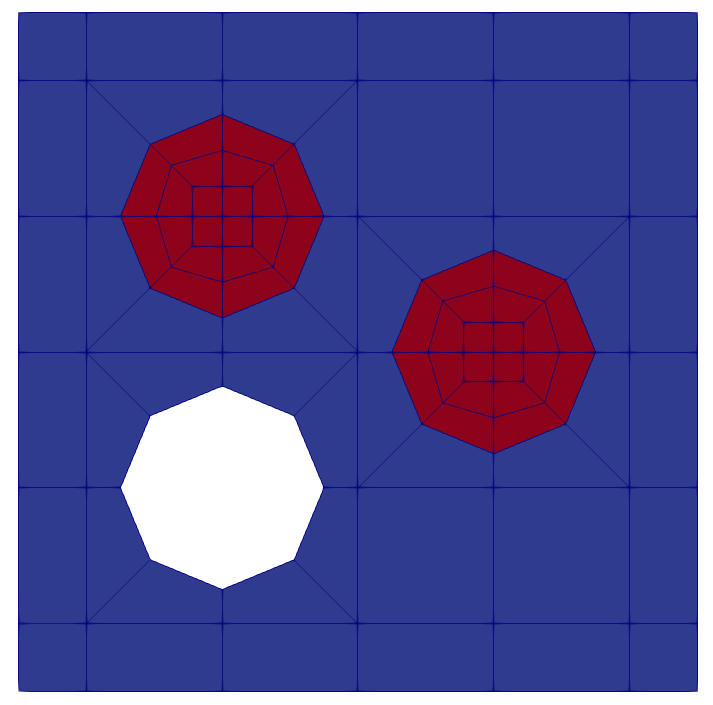
\includegraphics[width=\textwidth]{coarse_mesh.png}
      \caption{2D coarse mesh}
  \end{subfigure}
  \begin{subfigure}[b]{0.45\textwidth}
    \centering
    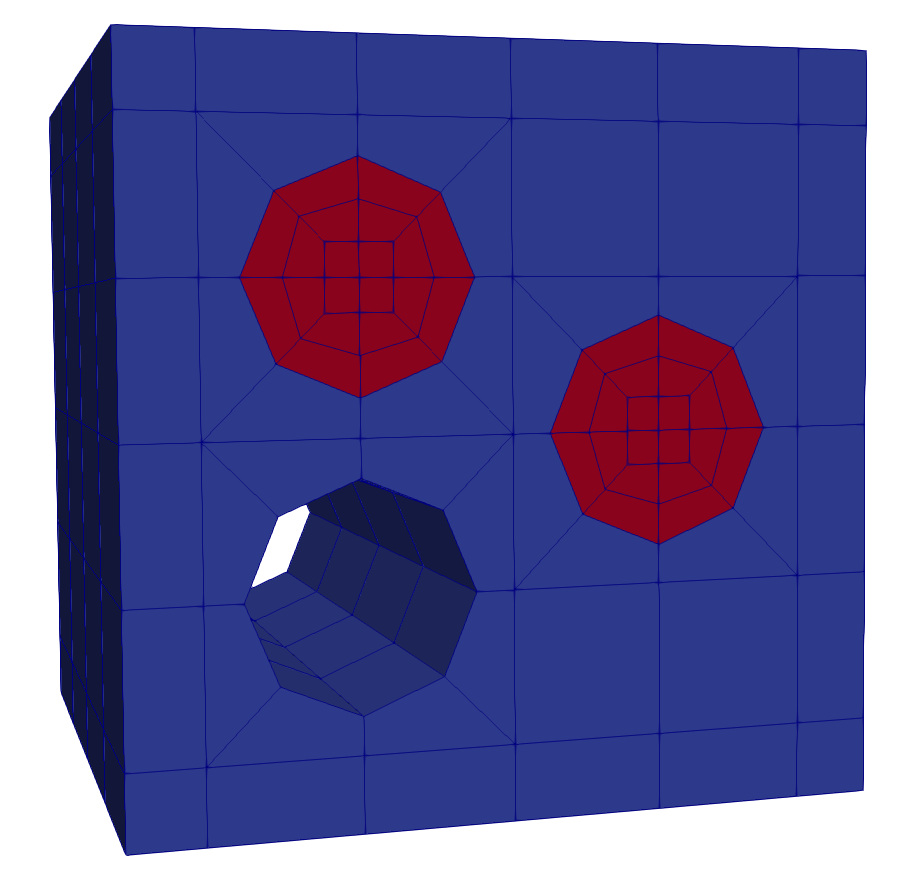
\includegraphics[width=\textwidth]{coarse_mesh_3d.png}
    \caption{3D coarse mesh}
  \end{subfigure}
  \caption{Heterogeneous material.}%
  \label{fig:miehe}
\end{figure}

\begin{figure}[!ht]
  \centering
  \begin{subfigure}[b]{0.8\textwidth}
    \centering
    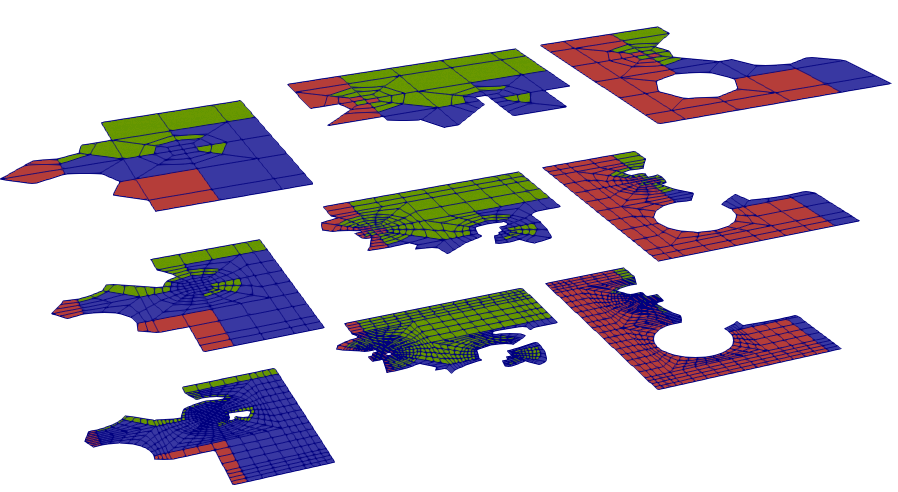
\includegraphics[width=\textwidth]{gmg_2d.png}
    % \caption{2D multigrid mesh with 2 global refinements}
  \end{subfigure}
  \caption{2D multigrid mesh after two global refinements distributed into three MPI processes. Color indicate the process owning the element.}%
  \label{fig:miehe_gmg}
\end{figure}

\begin{figure}[!ht]
  \centering
  \begin{subfigure}[b]{0.45\textwidth}
      \centering
      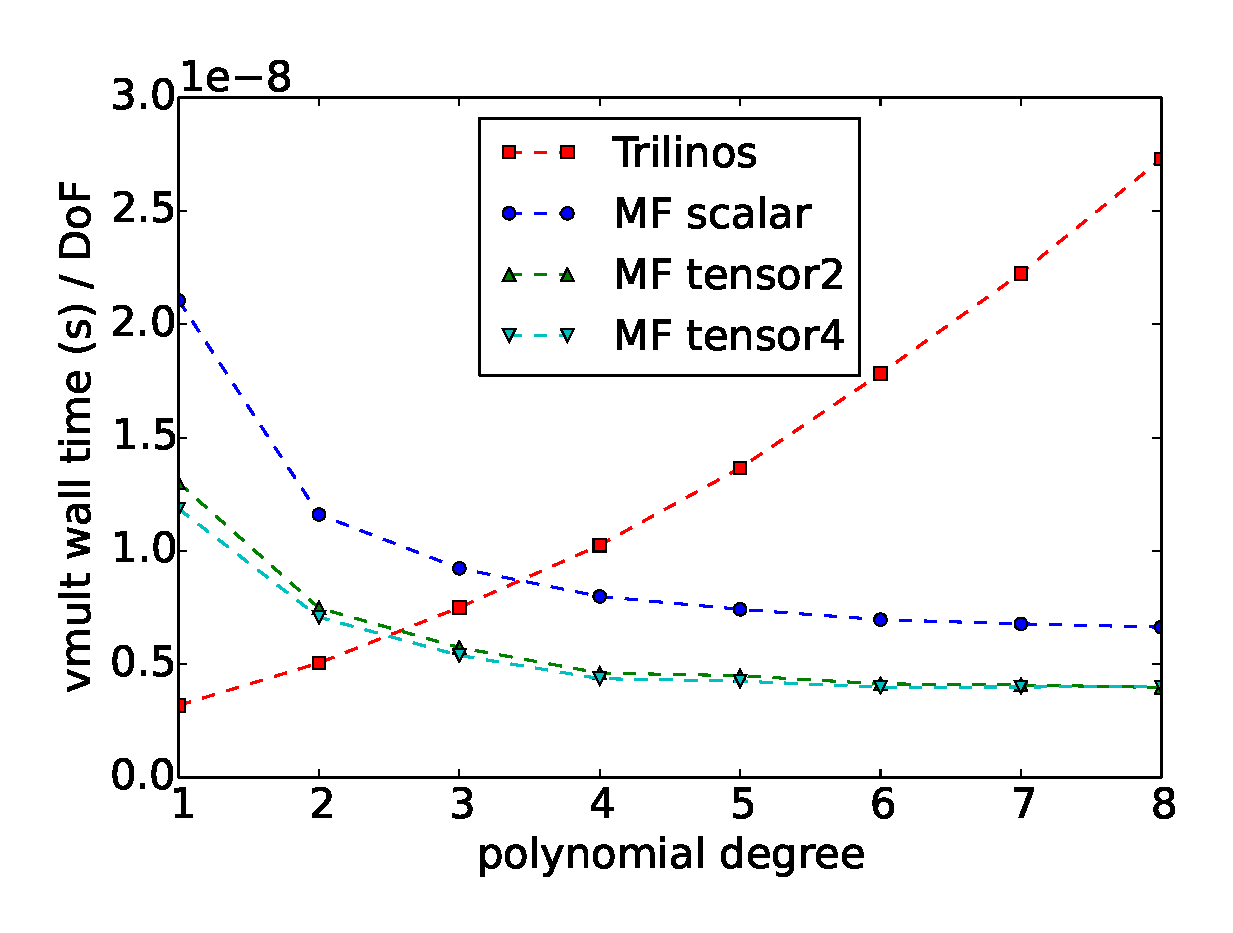
\includegraphics[width=\textwidth]{Emmy_RRZE_timing2d.eps}
      \caption{vmult 2D}
      \label{fig:benchmark_miehe_Emmy_vmult2}
  \end{subfigure}
  \begin{subfigure}[b]{0.45\textwidth}
    \centering
    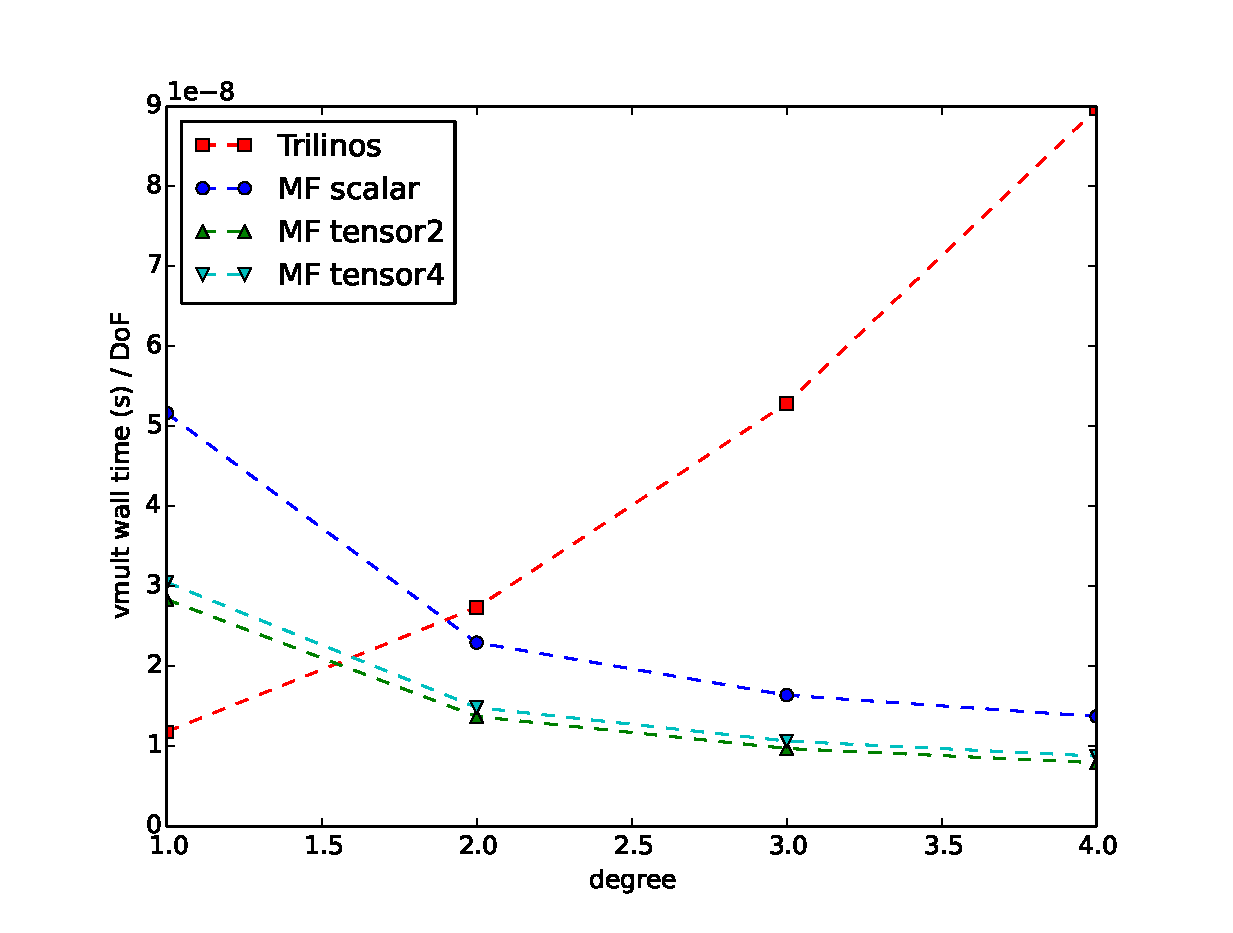
\includegraphics[width=\textwidth]{Emmy_RRZE_timing3d.eps}
    \caption{vmult 3D}
    \label{fig:benchmark_miehe_Emmy_vmult3}
  \end{subfigure}
  ~
  \begin{subfigure}[b]{0.45\textwidth}
      \centering
      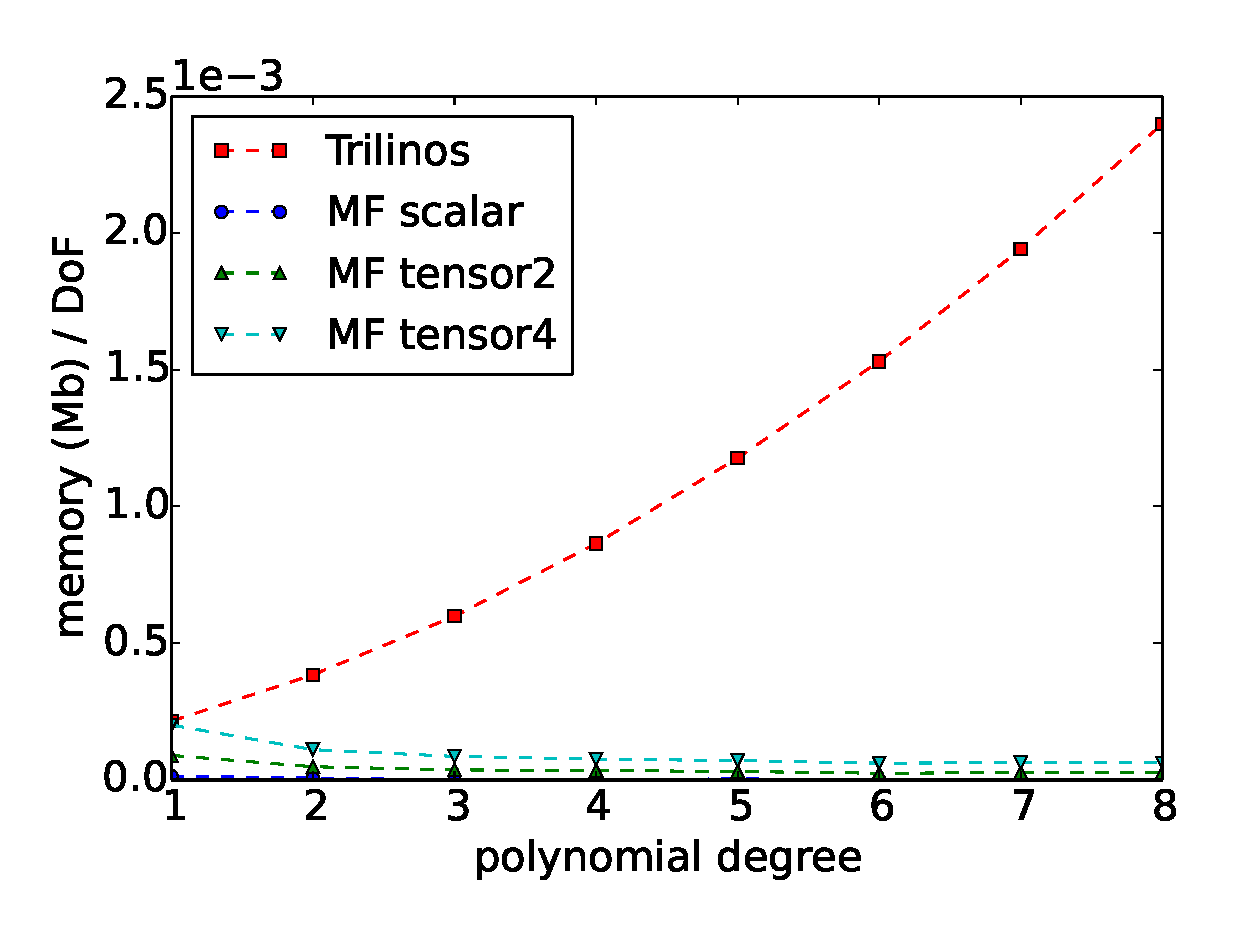
\includegraphics[width=\textwidth]{Emmy_RRZE_memory2d.eps}
      \caption{memory consumption 2D}
      \label{fig:benchmark_miehe_Emmy_memory2}
  \end{subfigure}
  \begin{subfigure}[b]{0.45\textwidth}
    \centering
    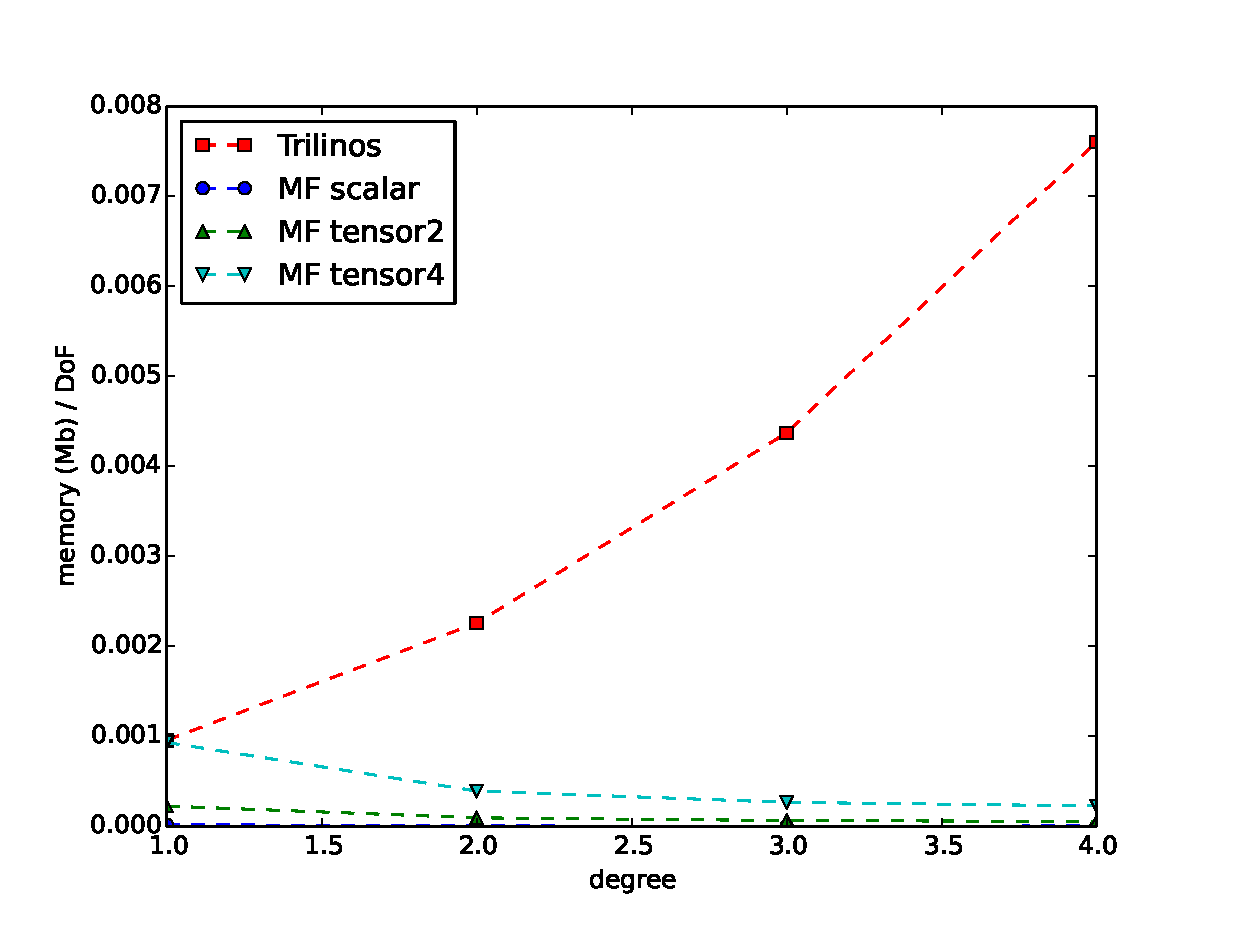
\includegraphics[width=\textwidth]{Emmy_RRZE_memory3d.eps}
    \caption{memory consumption 3D}
    \label{fig:benchmark_miehe_Emmy_memory3}
  \end{subfigure}
  ~
  \begin{subfigure}[b]{0.45\textwidth}
    \centering
    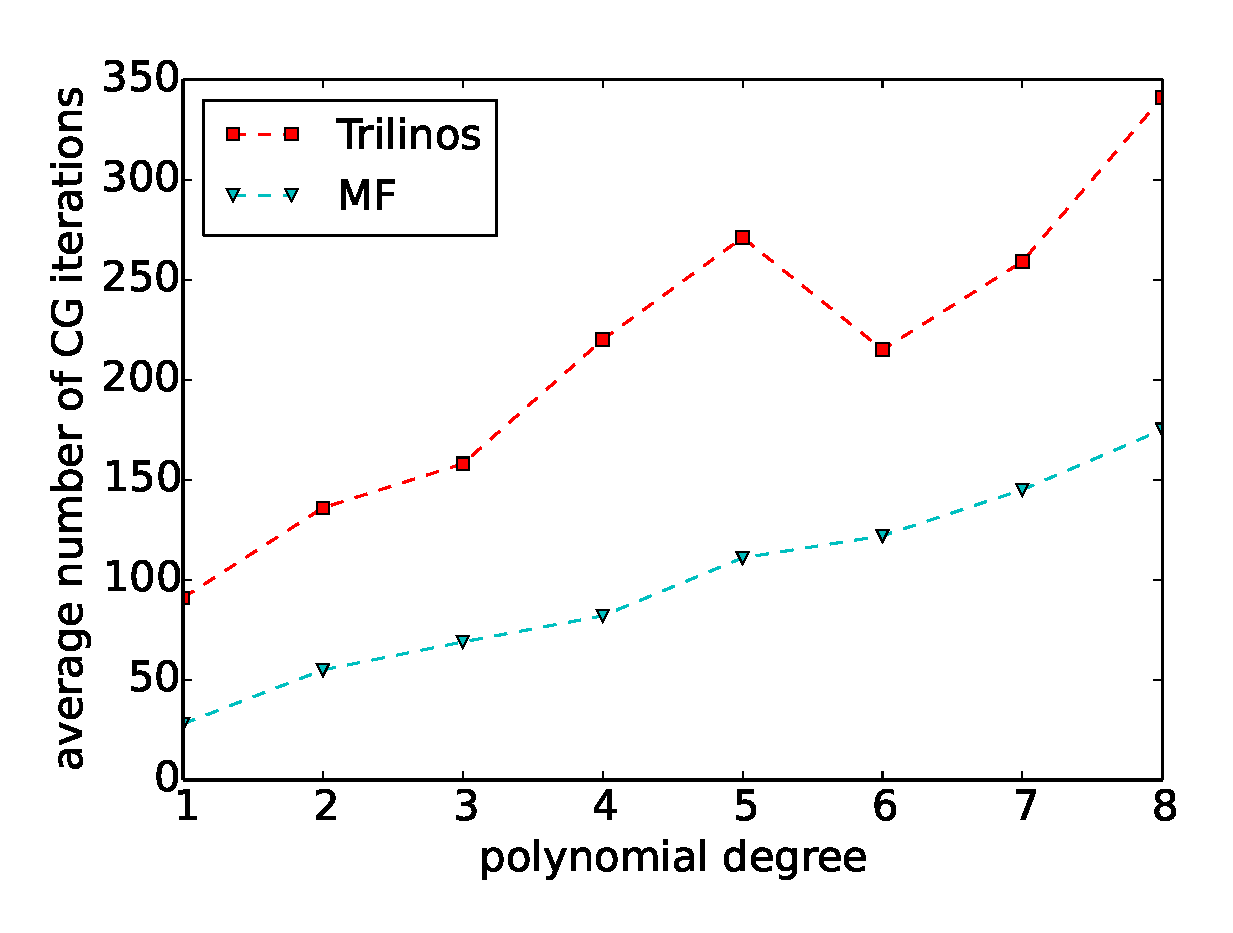
\includegraphics[width=\textwidth]{Emmy_RRZE_cg2d.eps}
    \caption{CG iterations 2D}
    \label{fig:benchmark_miehe_Emmy_cg2}
  \end{subfigure}
  \begin{subfigure}[b]{0.45\textwidth}
    \centering
    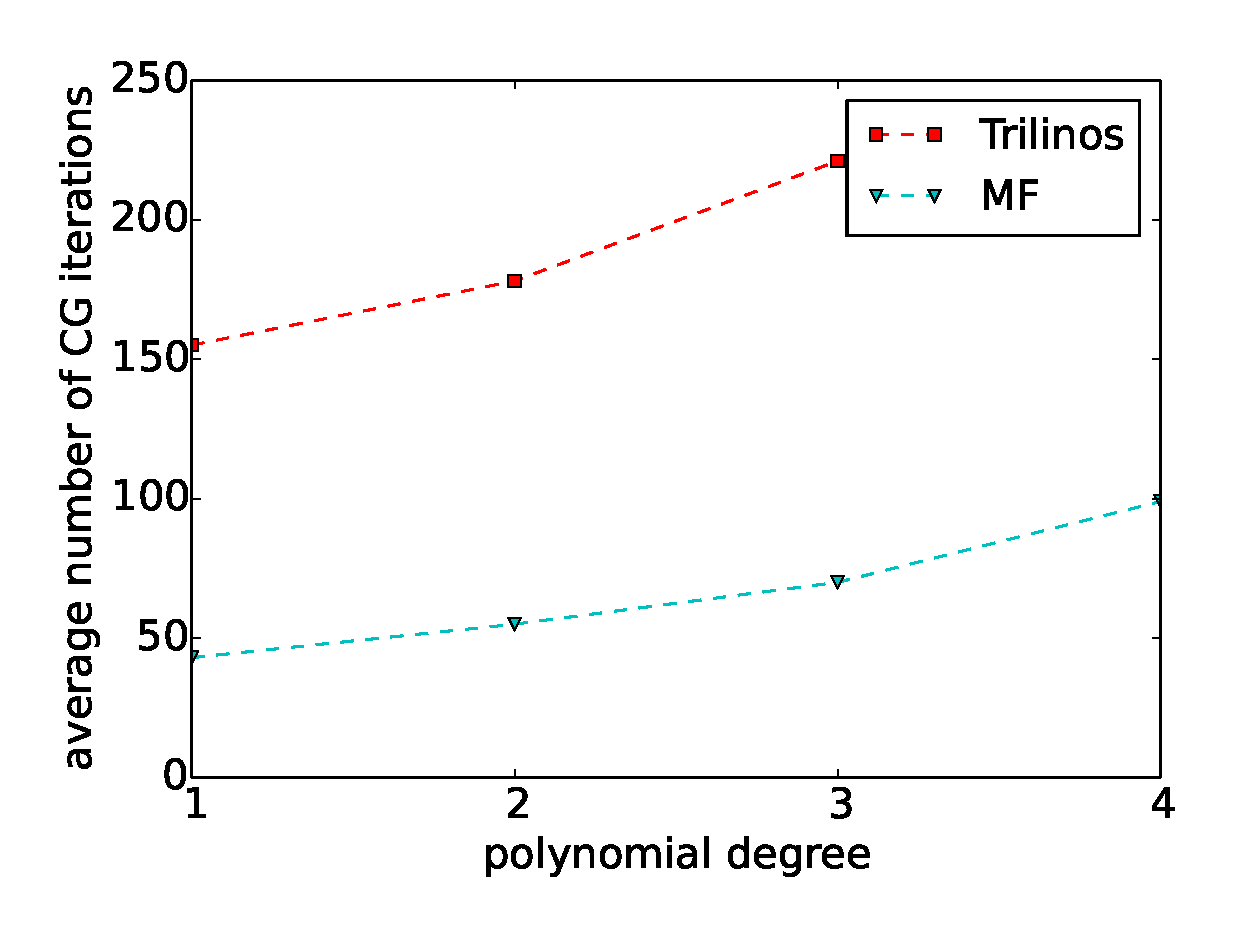
\includegraphics[width=\textwidth]{Emmy_RRZE_cg3d.eps}
    \caption{CG iterations 3D}
    \label{fig:benchmark_miehe_Emmy_cg3}
  \end{subfigure}
  ~
  \begin{subfigure}[b]{0.45\textwidth}
    \centering
    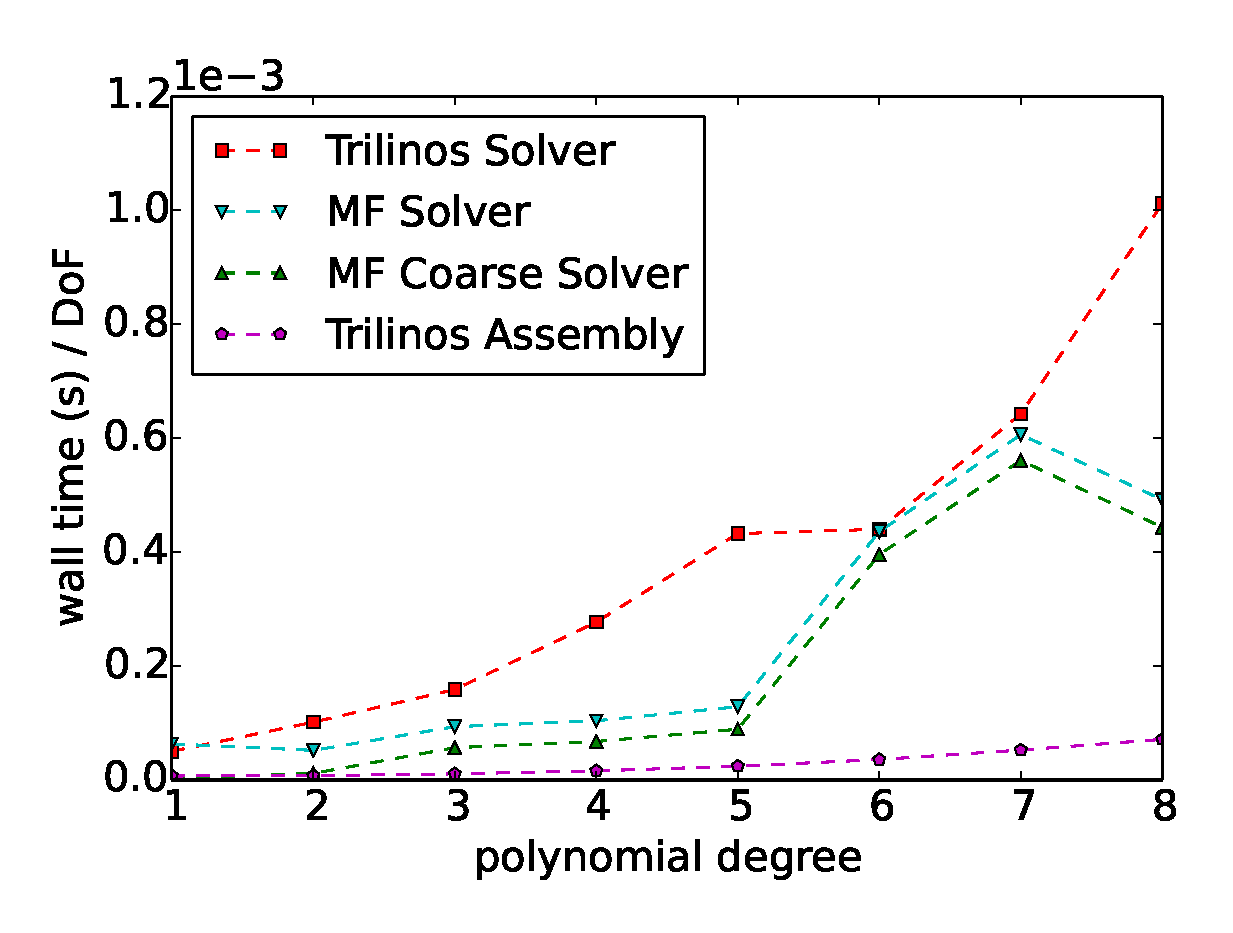
\includegraphics[width=\textwidth]{Emmy_RRZE_solver2d.eps}
    \caption{CG solution time 2D}
    \label{fig:benchmark_miehe_Emmy_sol2}
  \end{subfigure}
  \begin{subfigure}[b]{0.45\textwidth}
    \centering
    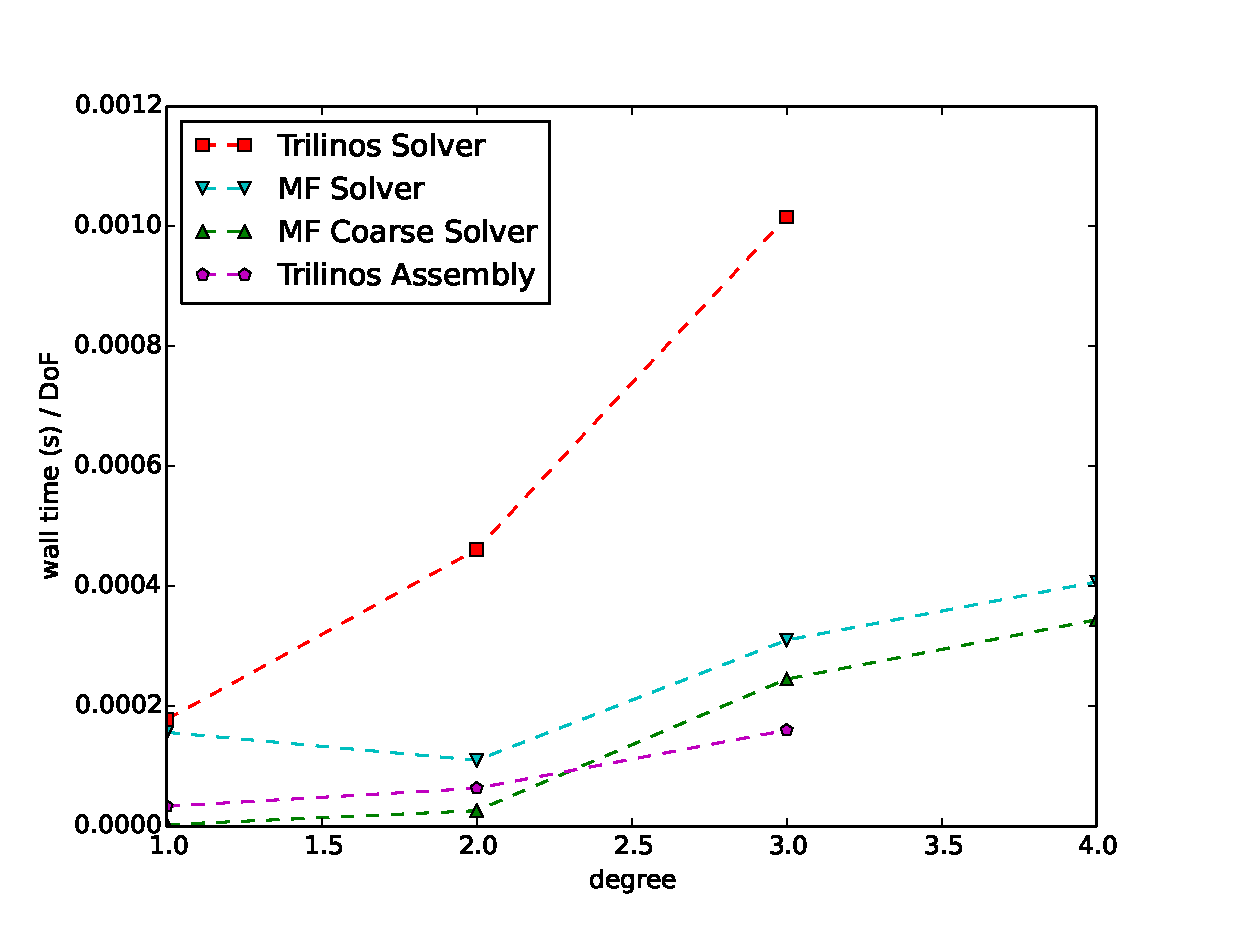
\includegraphics[width=\textwidth]{Emmy_RRZE_solver3d.eps}
    \caption{CG solution time 3D}
    \label{fig:benchmark_miehe_Emmy_sol3}
  \end{subfigure}
  \caption{Emmy cluster, RRZE.}%
  \label{fig:benchmark_miehe_Emmy}
\end{figure}

\begin{figure}[!ht]
  \centering
  \begin{subfigure}[b]{0.45\textwidth}
      \centering
      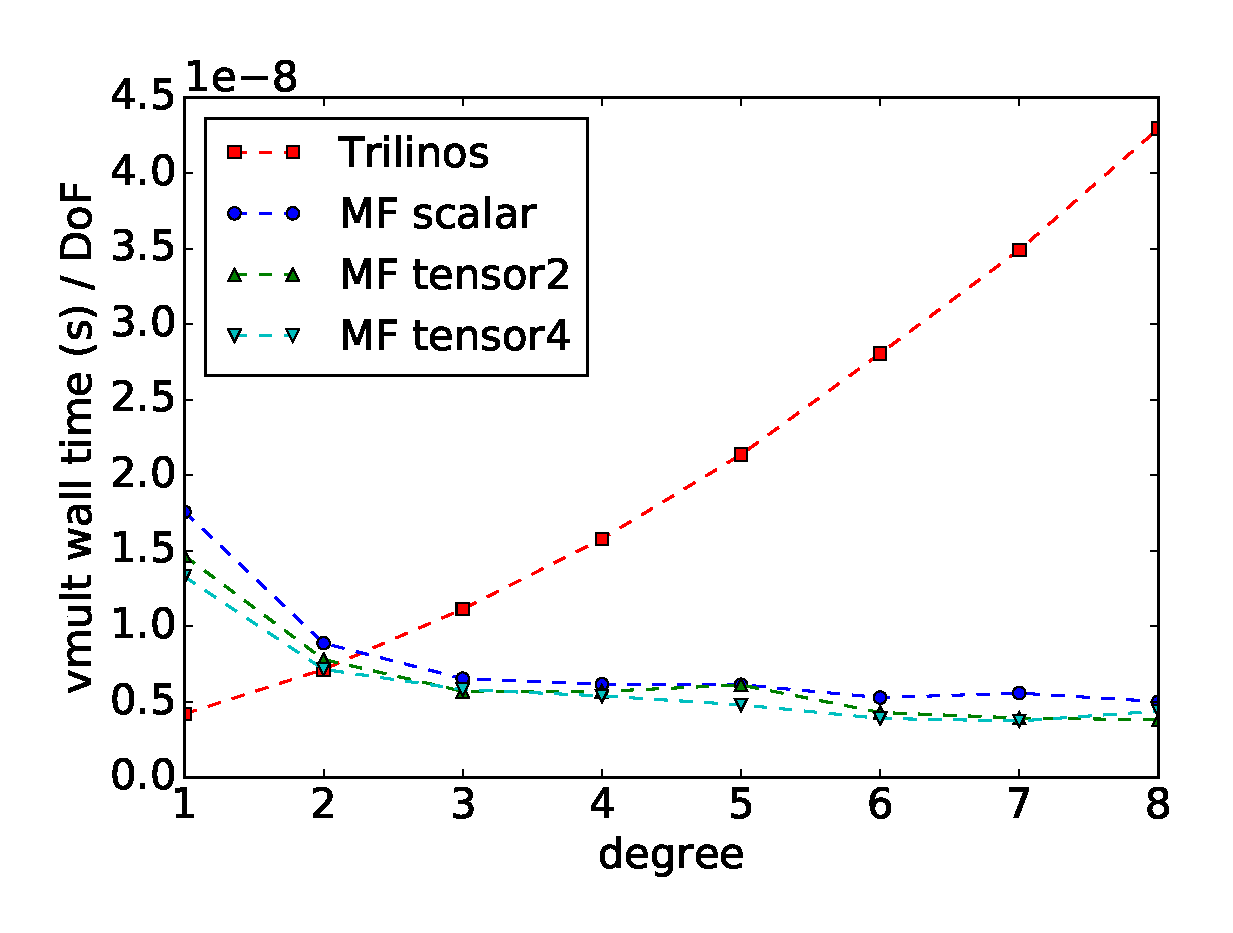
\includegraphics[width=\textwidth]{IWR_timing2d.eps}
      \caption{vmult 2D}
      \label{fig:benchmark_miehe_IWR_vmult2}
  \end{subfigure}
  \begin{subfigure}[b]{0.45\textwidth}
    \centering
    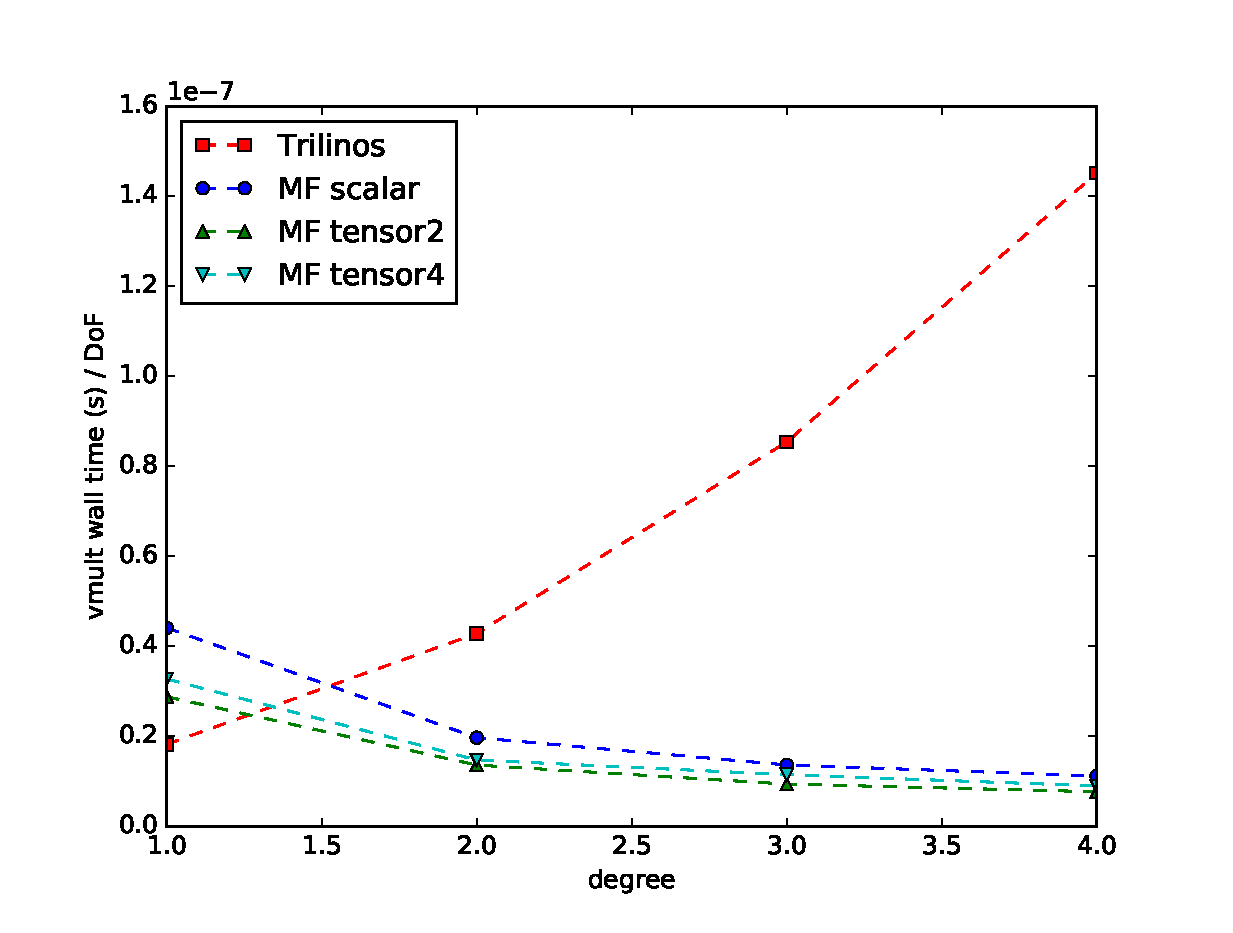
\includegraphics[width=\textwidth]{IWR_timing3d.eps}
    \caption{vmult 3D}
    \label{fig:benchmark_miehe_IWR_vmult3}
  \end{subfigure}
  ~
  \begin{subfigure}[b]{0.45\textwidth}
      \centering
      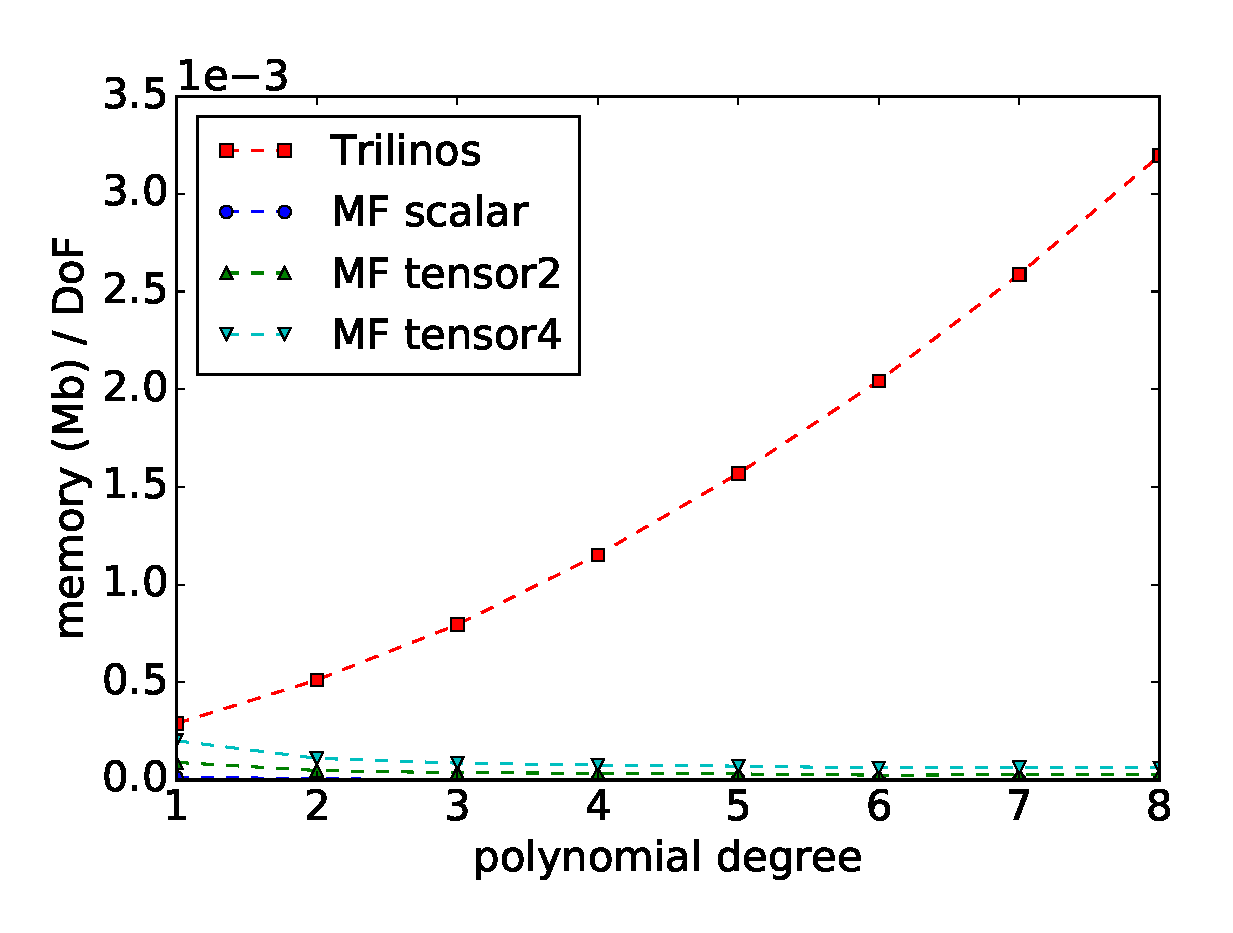
\includegraphics[width=\textwidth]{IWR_memory2d.eps}
      \caption{memory consumption 2D}
      \label{fig:benchmark_miehe_IWR_memory2}
  \end{subfigure}
  \begin{subfigure}[b]{0.45\textwidth}
    \centering
    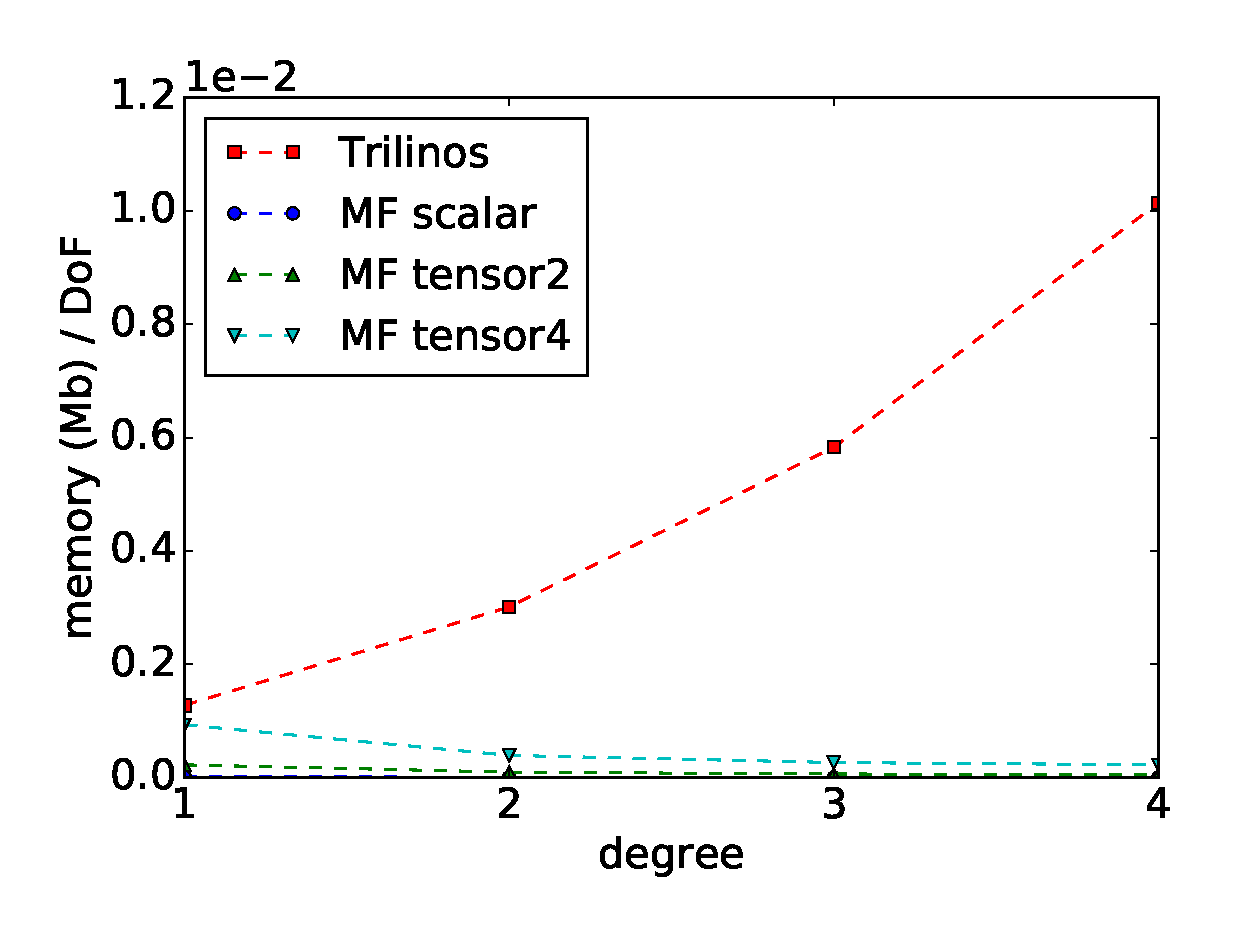
\includegraphics[width=\textwidth]{IWR_memory3d.eps}
    \caption{memory consumption 3D}
    \label{fig:benchmark_miehe_IWR_memory3}
  \end{subfigure}
  ~
  \begin{subfigure}[b]{0.45\textwidth}
    \centering
    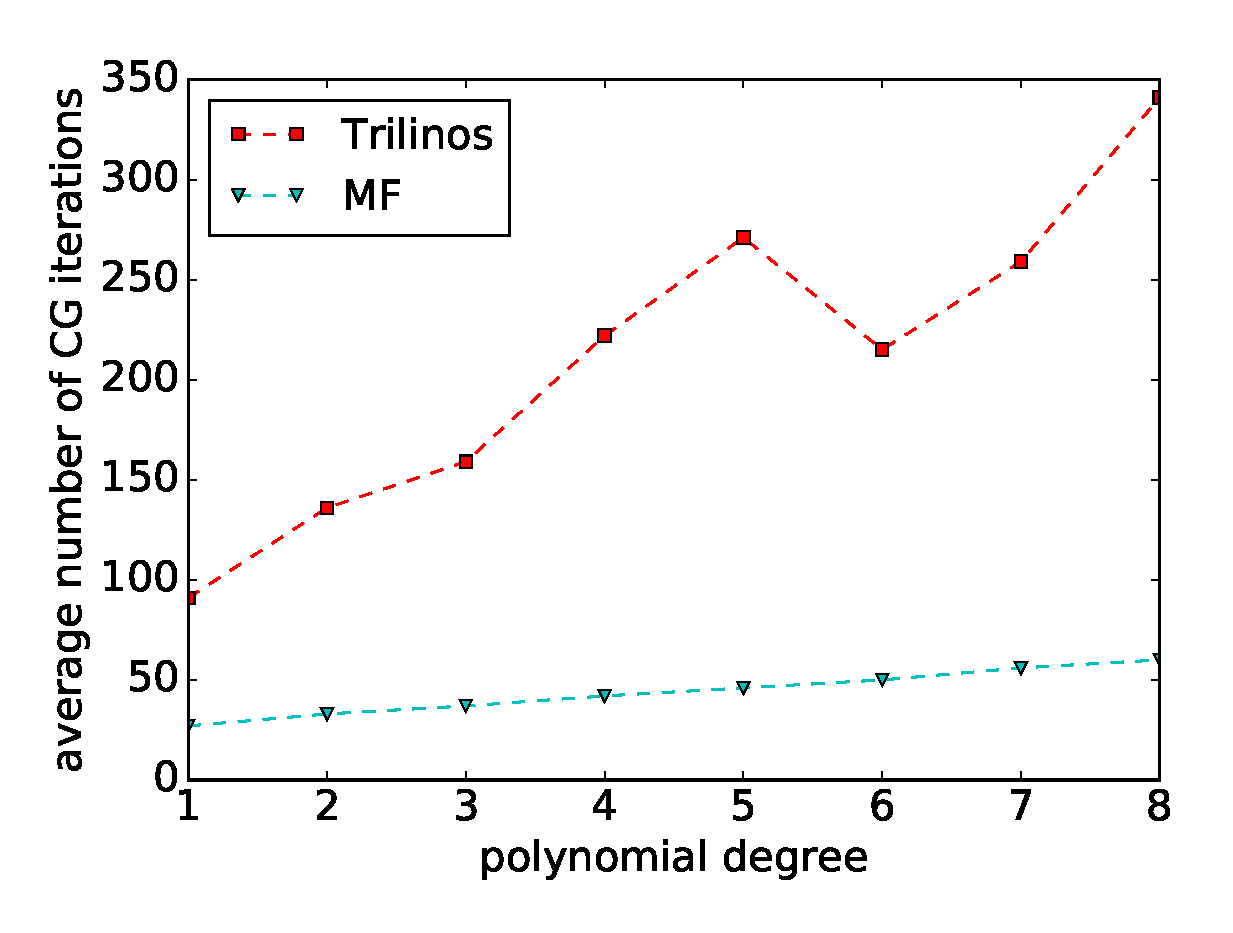
\includegraphics[width=\textwidth]{IWR_cg2d.eps}
    \caption{CG iterations 2D}
    \label{fig:benchmark_miehe_IWR_cg2}
  \end{subfigure}
  \begin{subfigure}[b]{0.45\textwidth}
    \centering
    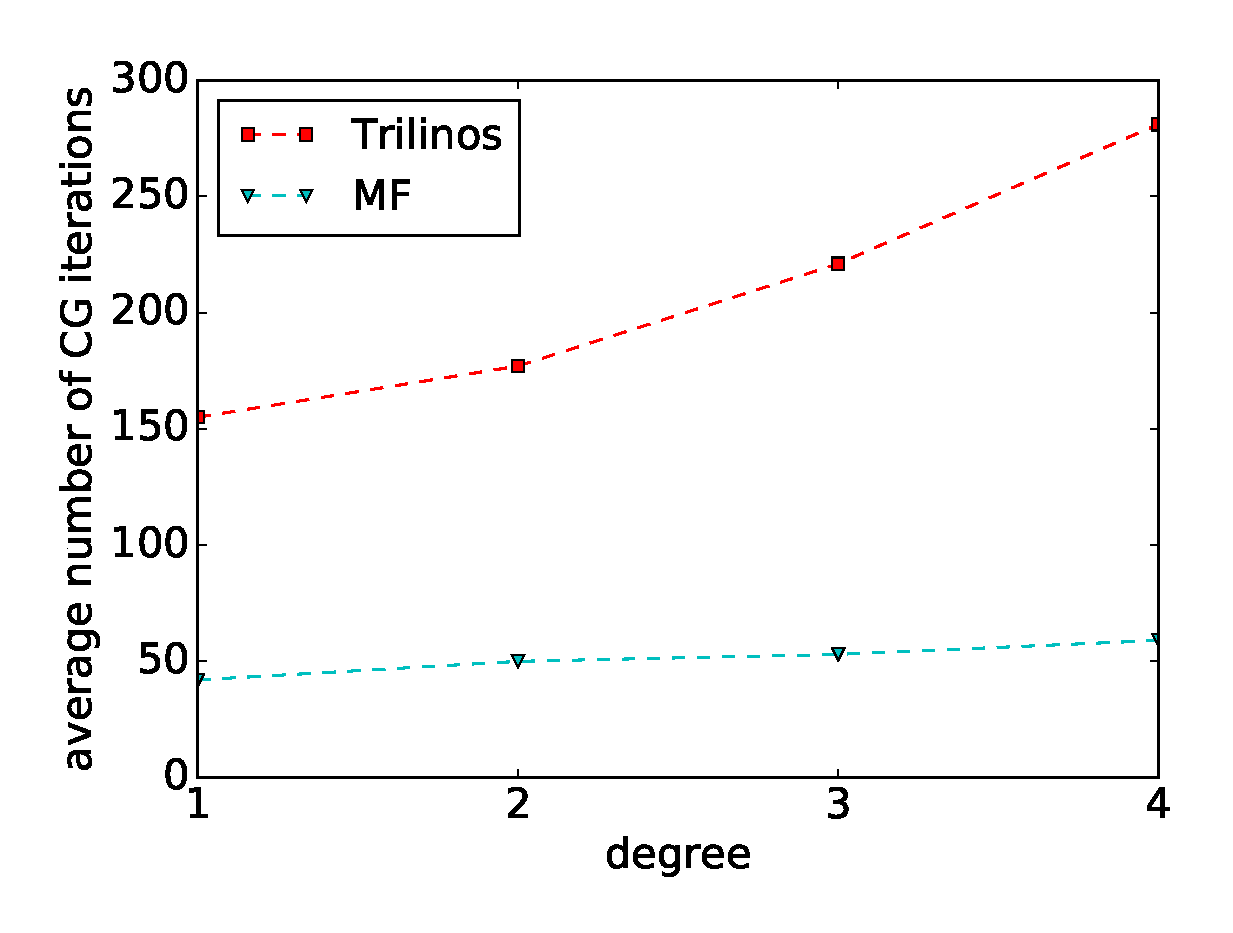
\includegraphics[width=\textwidth]{IWR_cg3d.eps}
    \caption{CG iterations 3D}
    \label{fig:benchmark_miehe_IWR_cg3}
  \end{subfigure}
  ~
  \begin{subfigure}[b]{0.45\textwidth}
    \centering
    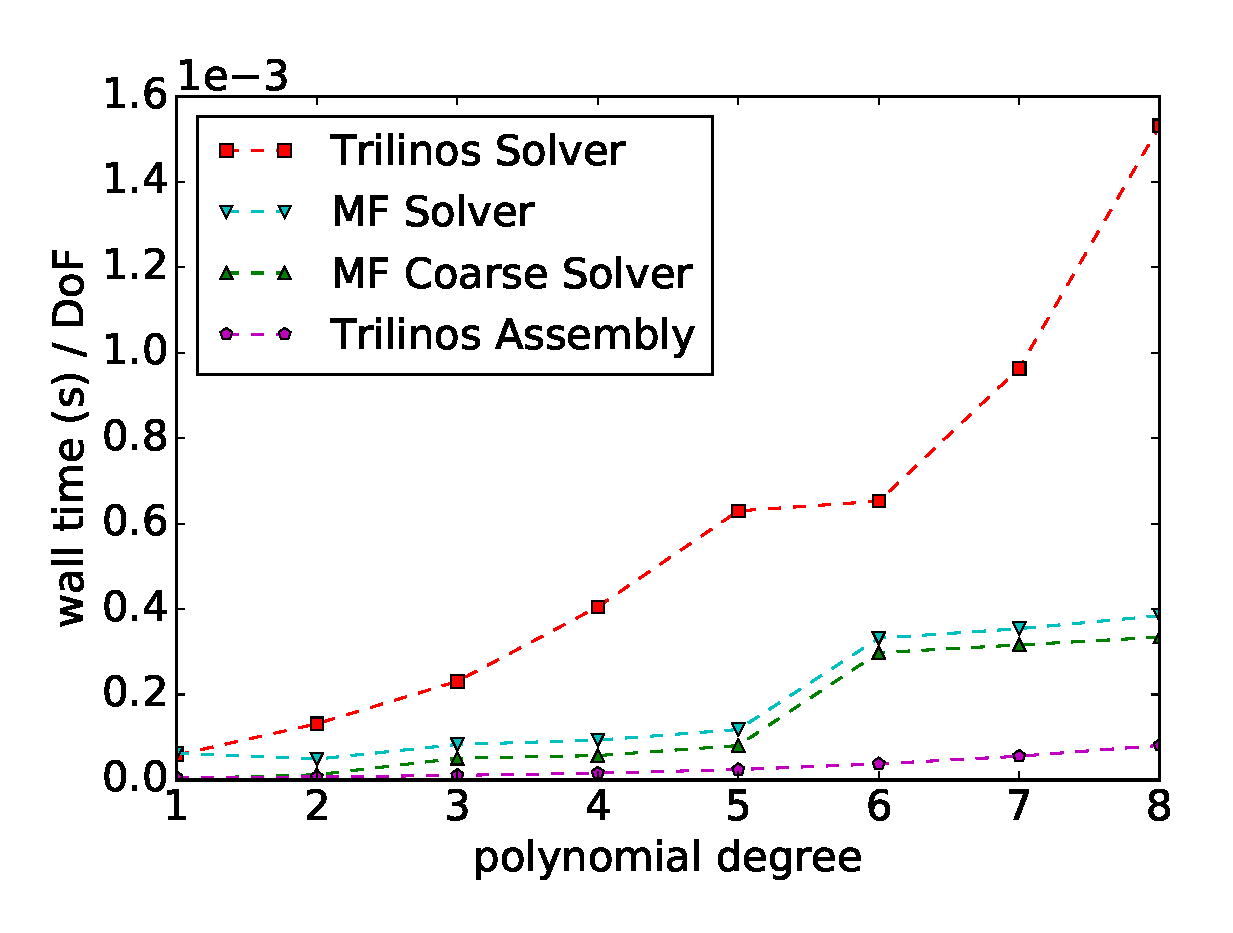
\includegraphics[width=\textwidth]{IWR_solver2d.eps}
    \caption{CG solution time 2D}
    \label{fig:benchmark_miehe_IWR_sol2}
  \end{subfigure}
  \begin{subfigure}[b]{0.45\textwidth}
    \centering
    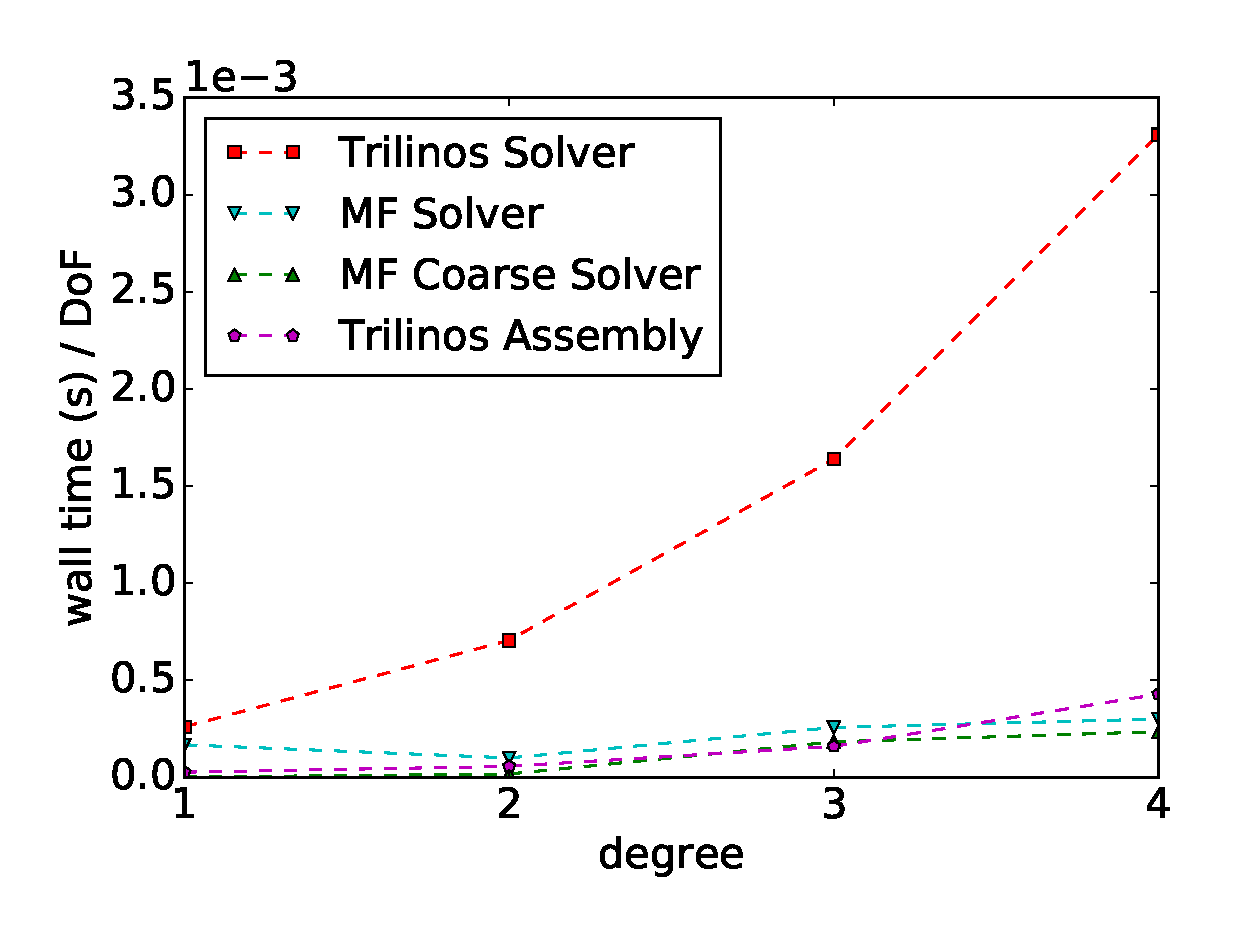
\includegraphics[width=\textwidth]{IWR_solver3d.eps}
    \caption{CG solution time 3D}
    \label{fig:benchmark_miehe_IWR_sol3}
  \end{subfigure}
  \caption{IWR cluster.}%
  \label{fig:benchmark_miehe_IWR}
\end{figure}


\section{Summary and Conclusions}
\label{sec:summary}

In this contribution we proposed and numerically investigated several matrix-free implementations of tangent operators for fine-strain elasticity of heterogeneous materials.
The implementation which caches the fourth order material tangent together with the second order Kirchhoff stress was shown to be faster than the matrix-based approach for quadratic elements in 3D and cubic in 3D.
This indicates that the matrix-free implementation of tangent operator can be applied any constitutive model which operates with the material tangent on quadrature point level.

We also studies the performance of the GMG preconditioner with standard geometric transfer operations between each level. The GMG was applied to heterogeneous material assuming that the coarsest level can provide adequate discretization of heterogeneity. The numerical studies indicate that the proposed preconditioner lead to the solution approach that is faster than the matrix-based algebraic multigrid preconditioner for moderate polynomial degrees. However the considerable amount of time is spent in the coarse level solver. Therefore our future work will be focused on extending this proposed here matrix-free multigrid solution approach to homogenization based transfer operators \cite{Miehe2007}. We are also interested  extending these methods to incompressible three-field formulation.

\section*{Acknowledgements}

D.~Davydov acknowledge the financial support of the German Research Foundation (DFG), grant DA 1664/2-1
and the Competence Network for Technical and Scientific High Performance Computing in Bavaria (KONWIHR).

D.~Davydov, D.~Arndt and J-P.~Pelteret are grateful to Jed Brown (CU Boulder) and Veselin Dobrev (Lawrence Livermore National Laboratory) for a fruitful discussion on matrix-free operator evaluation approaches.

D.~Arndt was supported by the German Research Foundation (DFG) under the project ``High-order discontinuous
Galerkin for the exa-scale'' (\mbox{ExaDG}) within the priority program ``Software
for Exascale Computing'' (SPPEXA).

{\color{red}
J-P.~Pelteret was supported by the European Research Council (ERC) through
the Advanced Grant 289049 MOCOPOLY.(?)
}

P.~Steinmann acknowledges the support of the Cluster of Excellence Engineering of Advanced Materials (EAM) which made this collaboration possible.

\section*{Bibliography}

\bibliographystyle{elsarticle-num}
\bibliography{bibliography}

\end{document}
